% !TeX root = bagrut-806.tex

\selectlanguage{hebrew}

\chapter{תנועה והספק}

%%%%%%%%%%%%%%%%%%%%%%%%%%%%%%%%%%%%%%%%%%%%%%%%%%%%%%%%%%%%%%%%

\section{קיץ תשע"ח מועד ב}

\begin{center}
\selectlanguage{english}
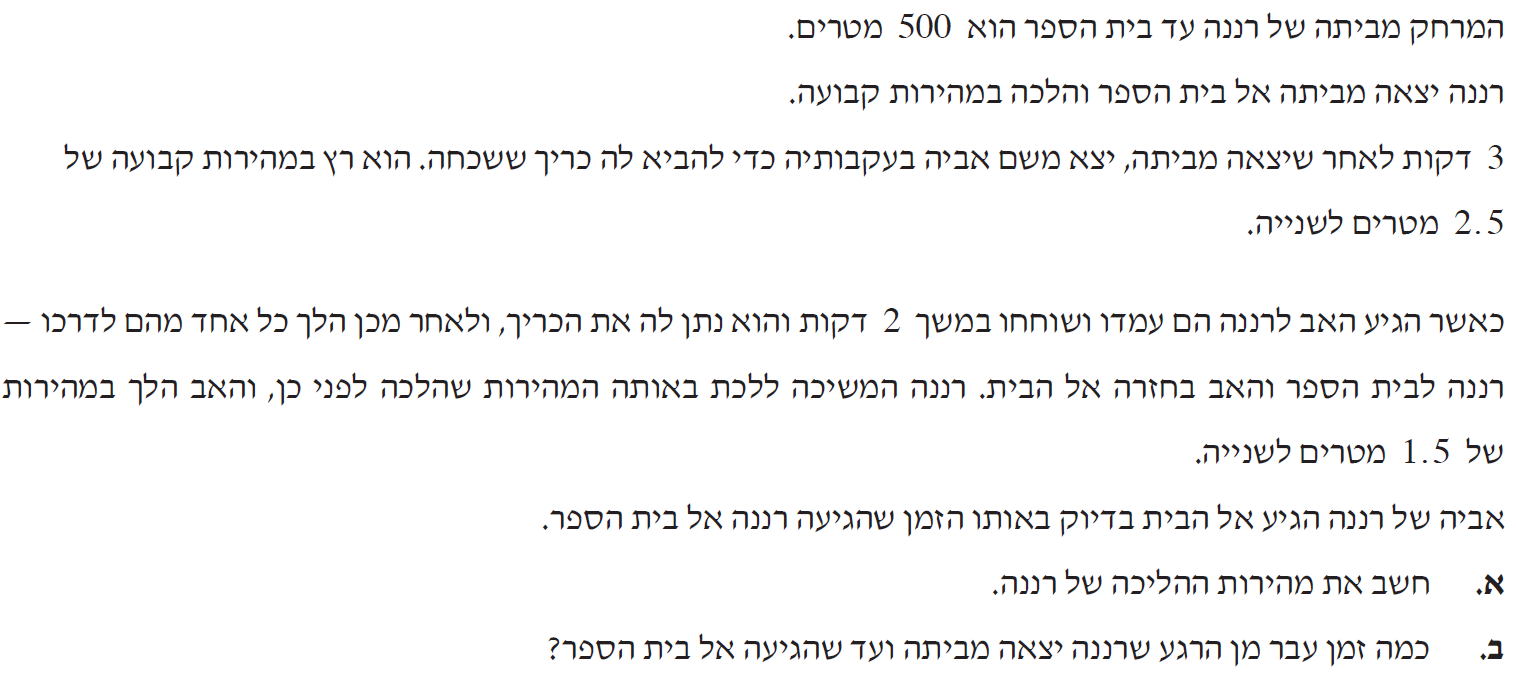
\includegraphics[width=\textwidth]{summer-2018b-1}
\end{center}

\begin{center}
\selectlanguage{english}
\begin{tikzpicture}
\draw (0,0) node[left] {$0$ } -- (10,0);
\node at (-.45,0.5) {
\R{בית}
};
\draw (0,0) -- (0,6) node[left] {$500$};
\node at (-.84,5.5) {
\R{בית ספר}
};
\draw[dashed] (0,6) -- (10,6);
\draw[thick] (0,0) -- node[above left] {
\R{רננה}
} (4.5,3);
\draw[thick] (2,0) -- node[above right,xshift=10pt,near start] {
\R{אבא}
} (4.5,3);
\draw[thick] (4.5,3) -- node[above] {
\R{רננה ואבא}
} (7,3);
\draw[thick] (7,3) -- node[above right] {
\R{אבא}
} (10,0);
\draw[thick] (7,3) -- node[above left] {
\R{רננה}
} (10,6);
\fill (4.5,3) circle [radius=2pt];
\fill (0,0) circle [radius=2pt];
\fill (2,0) circle [radius=2pt];
\fill (4.5,0) circle [radius=2pt];
\fill (7,0) circle [radius=2pt];
\fill (7,3) circle [radius=2pt];
\fill (10,0) circle [radius=2pt];
\fill (10,6) circle [radius=2pt];
\draw[dashed] (10,6) -- (10,0);
\draw[dashed] (4.5,3) -- (4.5,0);
\draw[dashed] (7,3) -- (7,0);
\draw[<->] (0,-5mm) -- node[fill=white] {$180$} (2,-5mm);
\draw[<->] (2,-5mm) -- node[fill=white] {$t$} (4.5,-5mm);
\draw[<->] (4.5,-5mm) -- node[fill=white] {$120$} (7,-5mm);
\draw[<->] (7,-5mm) -- node[fill=white] {$t'=\frac{5}{3}t$} (10,-5mm);
\end{tikzpicture}
\end{center}

\vspace*{-1ex}

נסמן:
$=v$
מהירות ההליכה של רננה,
$=t$
הזמן עד למפגש בין רננה לאביה,
$=t'$
הזמן מהפרידה בין רננה לאביה ועד ששניהם מגיעים ליעדם.

מהתרשים אפשר לראות שוויון בין מרחקים: רננה ואבא עד למפגש, אבא אל המפגש ובחזרה, וכן, שהמרחק לבית הספר מורכב משני קטעים שרננה הלכה. תחילה נשווה את המרחקים שאבא עובר מהבית עד למפגש ובחזרה כדי לקבל את
$t'$
כפונקציה של 
$t$:
\erh{14pt}
\begin{equationarray*}{rcl}
\frac{5}{2}t &=& \frac{3}{2}t'\\
t' &=& \frac{2}{3}\cdot\frac{5}{2}t = \frac{5}{3}t\,.
\end{equationarray*}

\np

\textbf{סעיף א}


עד למפגש המרחקים שעוברים רננה ואביה שווים:
\begin{equation}
v(t+180) = \frac{5}{2}t\,.\label{eq.rnna1}
\end{equation}
אנו זקוקים לשתי משוואות עם שני הנעלמים כדי למצוא את
$v$.
אי-אפשר למצוא משוואה שניה מהנתונים מהמפגש עד ליעדים, כי המרחקים והמהירויות לא בהכרח שווים. במקום זה נמצא דרך אחרת להשוות את המרחק שעוברים רננה ואבא מהבית עד למפגש.

עבור אבא נשתמש באותו ביטוי 
$\frac{5}{2}t$
שהשתמשנו במשוואה%
~\ref{eq.rnna1}.
עבור רננה נשים לב שניתן לחשב את המרחק כהפרש בין המרחק מהבית לבית הספר 
$(500)$
לבין המרחק שרננה עוברת מהמפגש ועד לבית הספר
$(vt')$:
\begin{equation}
\frac{5}{2}t = 500 - v\left(\frac{5}{3}t\right)\,.\label{eq.rnna2}
\end{equation}
ממשוואה%
~\ref{eq.rnna1}
ניתן למצוא משוואה עבור 
$t$:
\begin{equation}
t = \frac{360v}{5-2v}\,.\label{eq.rnna3}
\end{equation}
נציב את משוואה%
~\ref{eq.rnna3}
ב-%
~\ref{eq.rnna2}:
\[
500 - \frac{5}{3}v\left(\frac{360v}{5-2v}\right) = \frac{5}{2} \left(\frac{360v}{5-2v}\right)
\]
נפשט את המשוואה ונקבל משוואה ריבועית עבור
$v$:
\erh{2pt}
\begin{equationarray*}{rcl}
6v^2 + 19v - 25 &=& 0\\
(v-1)(6v+25)&=&0\,.
\end{equationarray*}
המהירות חייבת להיות חיובית ולכן הפרתון היחיד הוא
$v=1$.

\textbf{סעיף ב}


ממשוואה%
~\ref{eq.rnna1}
נקבל
$t=120$
ונסכם את פרקי הזמן על הציר האופקי בתרשים:
\[
180 + 120 + 120 + \frac{5}{3}\cdot 120 = 620
\]
שניות.

\medskip

\textbf{הערה}

שימו לב למלכודת שקל ליפול לתוכה: הזמנים נתונים בדקות והמהיריויות נתונות במטרים שנייה!


%%%%%%%%%%%%%%%%%%%%%%%%%%%%%%%%%%%%%%%%%%%%%%%%%%%%%%%%%%%%%%%%

\np

\section{קיץ תשע"ח מועד א}

\begin{center}
\selectlanguage{english}
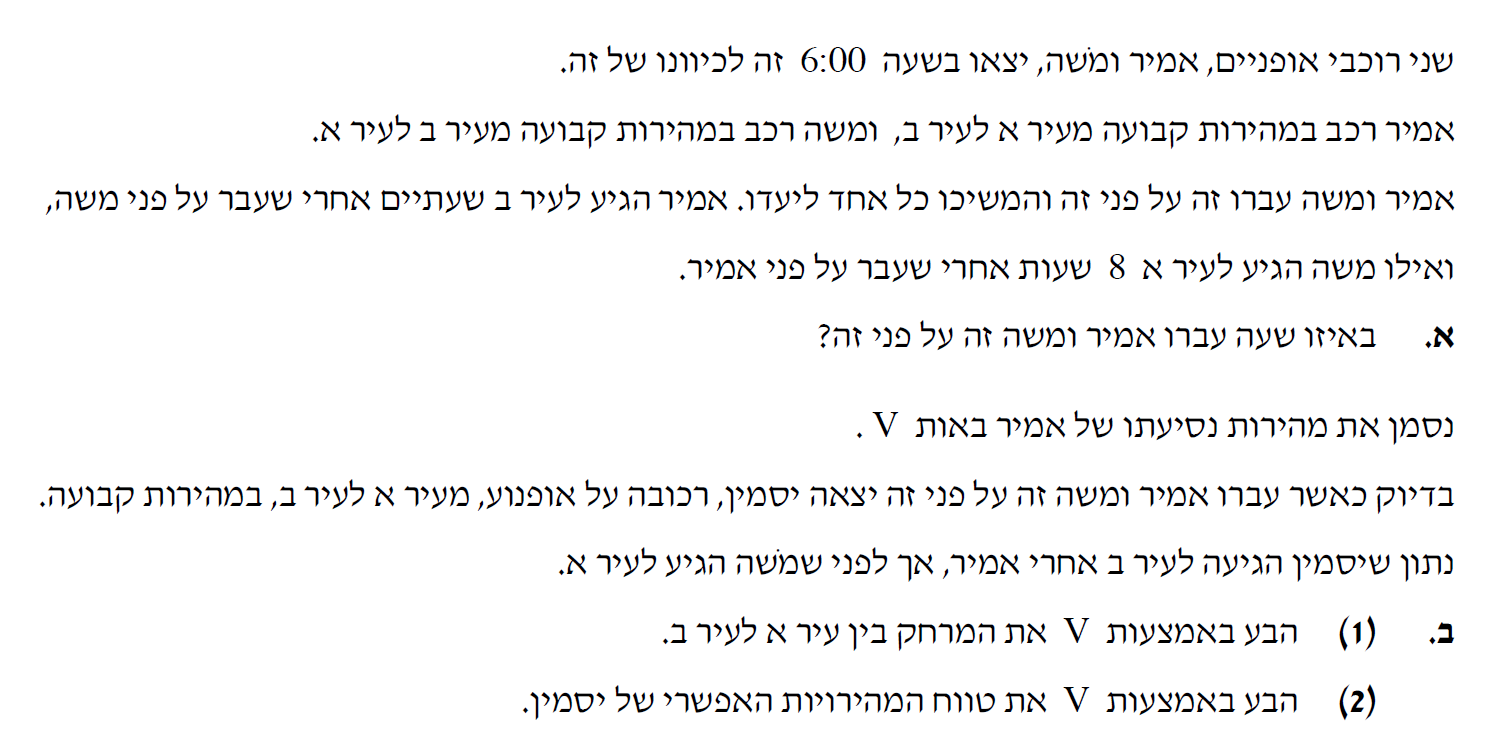
\includegraphics[width=\textwidth]{summer-2018a-1}
\end{center}

\begin{center}
\selectlanguage{english}
\begin{tikzpicture}[scale=.95]
\draw (0,0) node[left] {
\R{עיר א}
} node[below left,yshift=-6pt] {\p{06:00}} -- (10,0);
\draw (0,0) -- (0,6) node[left] {
\R{עיר ב}
};
\draw[dashed] (0,6) -- (10,6);
\draw[thick,name path=amir] (0,0) -- node[above left,near start] {
\R{אמיר}
} (6,6);
\draw[thick,name path=moshe] (0,6) -- node[above right,near start] {
\R{משה}
} (10,0);
\fill (0,6) circle [radius=2pt];
\fill (0,0) circle [radius=2pt];
\fill (6,6) circle [radius=2pt];
\fill (10,0) circle [radius=2pt];
\path[name intersections={of=amir and moshe,by=meeting}];
\fill (meeting) circle [radius=2pt];
\draw[dashed] (meeting) |- coordinate (meeting-time) (0,0);
\fill (meeting-time) circle [radius=2pt];
\draw[thick] (meeting-time) -- node[right,yshift=20pt,xshift=20pt] {
\R{יסמין}
} (8,6);
\fill (8,6) circle [radius=2pt];
\draw[dashed] (6,6) -- (6,0);
\draw[dashed] (8,6) -- (8,0);
\draw[dashed] (meeting) -| coordinate (meeting-distance) (0,0);
\fill (8,0) circle [radius=2pt];
\fill (meeting-distance) circle [radius=2pt];
\draw[<->] (0,-5mm) -- node[fill=white] {$t$} (meeting-time |- 0,-5mm);
\draw[<->] (meeting-time |- 0,-5mm) -- node[fill=white] {$2$} (6,-5mm);
\draw[<->] (meeting-time |- 0,-10mm) -- node[fill=white] {$8$} (10,-10mm);
\draw[<->] (meeting-time |- 0,-15mm) -- node[fill=white] {$t_y$} (8,-15mm);
\end{tikzpicture}
\end{center}

נסמן:
$=t$
הזמן עד ממפגש בין אמיר למשה,
$=t_y$
זמן הנסיעה של יסמין מעיר א לעיר ב, 
$=v_y,v_m,v_a$
המהירויות של אמיר, משה ויסמין.


\textbf{סעיף א}

מהתרשים מאוד עוזר לראות שיש
\textbf{שלושה}
ביטויים עבור המרחק בין הערים: )א( הרחק שנסע אמיר, )ב(המרחק שנסע משה, ו-)ג( סכום המרחקים שנסעו אמיר ומשה עד למפגש:
\[
tv_a + tv_m = (t+2) v_a = (t+8) v_m\,.
\]
משני הביטויים הראשונים אנו מקבלים:
\[
\frac{v_a}{v_m}=\frac{t}{2}\,.
\]

\np

נציב בשני הביטויים האחרונים:
\[
(t+2)\cdot \frac{tv_m}{2} = (t+8) v_m\,.
\]
$v_m$
מצטמצם ונקבל משוואה ריבועית
$t^2-16$
עם הפתרון חיובי 
$t=4$.

\textbf{שימו לב}

יש נטייה לעצור כאן כאשר חישבנו את הזמן 
$t$,
אבל עיון חוזר בשאלה מראה שהיא מבקשת את השעה של המפגש שהיא
\L{\p{10:00}}.
לאחר שפותרים בעייה יש לעיין שוב בשאלה כדי לוודא שאנו מספקים את התשובה הנדרשת.

\smallskip

\textbf{סעיף ב}

המרחק בין הערים הוא 
$(t+2)v_a$.
חישבנו ש-%
$t=4$
ולכן המרחק הוא
$6v_a=6V$
)הסימון הנתון 
$V$
שונה מ-%
$v_a$
שבחרתי בתחלית הפתרון(.


\smallskip

\textbf{סעיף ג}

נתון שיסמין מגיע לעיר ב אחרי אמיר ולפני משה. מהתרשים רואים ש:
\[
2 < t_y < 8\,.
\]
זמן הוא מרחק חלקי מהירות ואת המרחק חישבנו בסעיף ב:
\[
2 < \frac{6V}{v_j} < 8\,.
\]
מכאן ש:
\[
\frac{3}{4}v_a < v_j < 3v_a\,
\]
כי כיווני האי-שוויון מתחלפים עם היפוך השבר.

%%%%%%%%%%%%%%%%%%%%%%%%%%%%%%%%%%%%%%%%%%%%%%%%%%%%%%%%%%%%%%%%

\np

\section{חורף תשע"ח}

\begin{center}
\selectlanguage{english}
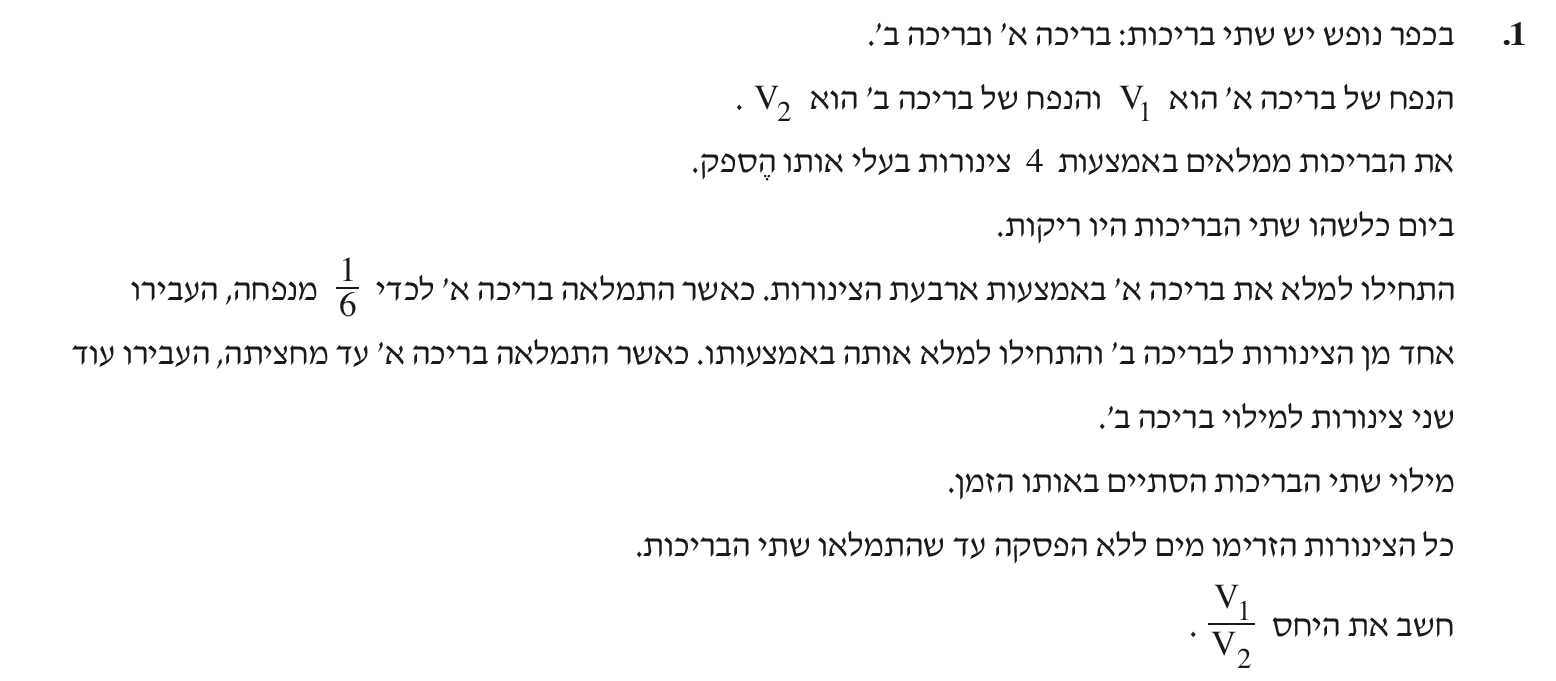
\includegraphics[width=\textwidth]{winter-2018-1}
\end{center}

\begin{center}
\selectlanguage{english}
\begin{tikzpicture}[scale=1]
\draw (0,0) node[left] {$0$} -- (10,0);
\draw (0,0) -- (0,6);
\node at (-.5,1) {$\frac{1}{6}V_1$};
\node at (-.5,3) {$\frac{1}{2}V_1$};
\node at (-.5,6) {$V_1$};

\fill (0,0) circle [radius=2pt];
\draw[dashed] (0,1) -- (1,1);
\draw (0,0) -- node[below,xshift=4pt] {$4x$} (1,1);
\fill (1,1) circle [radius=2pt];

\draw[dashed] (0,3) -- (4,3);
\draw (1,1) -- node[below,xshift=4pt] {$3x$} (4,3);
\fill (4,3) circle [radius=2pt];

\draw[dashed] (0,6) -- (10,6);
\draw (4,3) -- node[below,xshift=4pt] {$x$} (10,6);
\fill (10,6) circle [radius=2pt];

\draw[dashed] (1,1) -- (1,0);
\draw[dashed] (4,3) -- (4,0);
\draw[dashed] (10,6) -- (10,0);

\draw[<->] (10.5,0) -- node[fill=white] {$V_2$} (10.5,5.5);

\fill (1,0) circle [radius=2pt];
\draw (1,0) -- node[below,xshift=4pt] {$x$} (4,1);
\fill (4,1) circle [radius=2pt];
\draw (4,1) -- node[below,xshift=4pt] {$3x$} (10,5.5);
\fill (10,5.5) circle [radius=2pt];

\draw[<->] (0,-.5) -- node[fill=white] {$t_1$} (1,-.5);
\draw[<->] (1,-.5) -- node[fill=white] {$t_2$} (4,-.5);
\draw[<->] (4,-.5) -- node[fill=white] {$t_3$} (10,-.5);


\end{tikzpicture}
\end{center}


נסמן:
$=x$
קצב המילוי של כל צינור )"בעלי אותו הספק"(,
$=t_1, t_2, t_3$
פרקי הזמן בין העברת הצינורות.

הקו העליון בתרשים מתאר את המילוי של בריכה א, והקו התחתון מתאר את מילוי של בריכה ב. שימו לב שככל שיותר צינורות ממלאים בריכה, השיפוע של הקו תלול יותר.

יש לנו שלושה סוגים של נעלמים: 
$x$,
שלושת ה-%
$t_i$
ושני ה-%
$V_i$.
אם נצליח להיפטר מ-%
$x$
או מה-%
$t_i$,
השני יצטמצם כאשר נחלק את ה-%
$V_i$.

נתחיל עם משוואות ההספק עבור בריכה א, כאשר בכל פרק זמן ממלאים את ההפרשים של הנפחים, למשל, בזמן 
$t_2$
בריכה א מתמלאת מששית לחצי:

\np

\erh{12pt}
\begin{equationarray*}{rcl}
4x t_1 &=& \frac{1}{6}V_1\\
3x t_2 &=& \left(\frac{1}{2}-\frac{1}{6}\right)V_1\\
xt_3&=&\left(1-\frac{1}{2}\right)V_1\,.
\end{equationarray*}
נשתמש במשוואת כדי לחשב את פרקי הזמן כתלות בנפח בבריכה:
\erh{12pt}
\begin{equationarray*}{rcl}
t_1 &=& \frac{V_1}{24x}\\
t_2 &=& \frac{V_1}{9x}\\
t_3&=&\frac{V_1}{2x}\,.
\end{equationarray*}

מהתרשים רואים שאפשר לבטא את הנפח של
$V_2$
כסכום של שני חלקים: הנפח שמתמלא בפרק הזמן
$t_2$
והנפח המתמלא בפרק הזמן
$t_3$.
כאשר נציב את המשוואות שקבלנו עבור בפרקי הזמן, נקבל את הנפח של
$V_2$
כתלות ב-%
$V_1$
בלבד, כי המשתנה 
$x$ מצטמצם:
\erh{12pt}
\begin{equationarray*}{rcl}
V_2 &=& xt_2 + 3xt_3 = \frac{x V_1}{9x} + \frac{3x V_1}{2x}\ = \frac{29}{18}V_1\\
\frac{V_1}{V2} &=& \frac{18}{29}\,.
\end{equationarray*}

\textbf{הערה}

קיבלנו שהנפח של בריכה ב גדול מהנפח של בריכה א, עובדה שלא ידעתי כאשר ציירתי את התרשים עם נפח בריכה א גדול מנפח בריכה ב. אין לזה חשיבות. מטרת התרשים היא להציג את התסריט כדי שנוכל לכתוב את המשוואות הנכונות. 

פרט מעניין הוא שפרק הזמן הראשון
$t_1$
לא נחוץ לפתרון, כי המילוי של בריכה ב מתבצע בשני השלבים לאחר העברת הצינור הראשון.

%%%%%%%%%%%%%%%%%%%%%%%%%%%%%%%%%%%%%%%%%%%%%%%%%%%%%%%%%%%%%%%%

\np

\section{קיץ תשע"ז מועד ב}

\begin{center}
\selectlanguage{english}
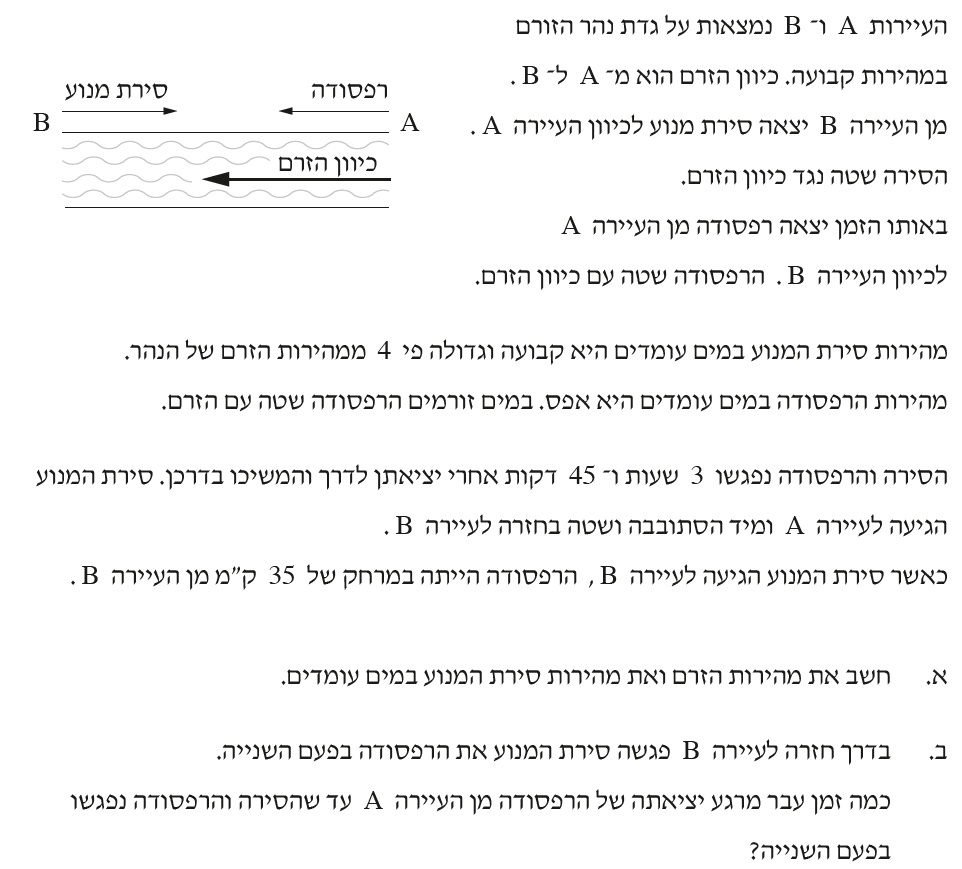
\includegraphics[width=.9\textwidth]{summer-2017b-1}
\end{center}

\vspace{-2ex}

\textbf{סעיף א}

\vspace{-3ex}

\begin{center}
\selectlanguage{english}
\begin{tikzpicture}[scale=.9]
\draw[name path=xaxis] (0,0) node[below left] {$A$} -- (10,0);
\draw (0,0) -- (0,6) node[above left] {$B$};
\draw[dashed] (0,6) -- (10,6);
\draw[thick,name path=raft] (0,0) -- node[left,near start,xshift=-4pt] {
\R{רפסודה}
} (10,4.5);
\draw[thick,name path=boat1] (0,6) -- node[right,near start,xshift=2pt] {
\R{סירה}
} (7,0);
\draw[thick,name path=boat2] (7,0) -- (10,6);
\path [name intersections={of=boat1 and raft,by=meeting1}];
\draw[dashed] (meeting1) |- coordinate (time) (0,0);
\draw[dashed] (meeting1) -| coordinate (distance) (0,0);
\draw[dashed] (10,0) -- (10,6);
\path[name path=t1] (7,0) -- (7,6);
\path [name intersections={of=raft and t1,by=a}];
\path [name intersections={of=raft and boat2,by=meeting2}];
\fill (meeting1) circle [radius=2pt];
\fill (meeting2) circle [radius=2pt];
\path [name path=t2] (meeting2) |- (0,0);
\path [name intersections={of=xaxis and t2,by=t2x}];
\fill (time) circle [radius=2pt];
\fill (0,0) circle [radius=2pt];
\fill (7,0) circle [radius=2pt];
\fill (10,6) circle [radius=2pt];
\fill (10,4.5) circle [radius=2pt];
\fill (0,6) circle [radius=2pt];
\fill (distance) circle [radius=2pt];
\draw[<->] (-.4,0) -- node[fill=white] {$d_r$} (distance -| -.4,0);
\draw[<->] (distance -| -.4,0) -- node[fill=white] {$d_s$} (-.4,6);
\draw[<->] (-.9,0) -- node[fill=white] {$d$} (-.9,6);
\draw[<->] (0,-.6) -- node[fill=white] { $15/4$} (time |- 0,-.6);
\draw[<->] (10.4,4.5) -- node[fill=white] { $35$} (10.4,6);
\end{tikzpicture}
\end{center}
נסמן:
$=d$
מרחק בין שני הנמלים,
$=d_r, d_s$
מרחקי ההפלגה של הסירה והרפסודה עד למפגש הראשון,
$=v_z$
מהירות הזרם,
$=v_s$
מהירות הסירה במים עומדים. בתרשים ציר הזמן הוא בשעות.

\np

הזמן עד למפגש הראשון שווה עבור הסירה והרפסודה ויחס המהירויות של הסירה והזרם ידוע, כך שנכתוב את משוואות התנועה עד למפגש. נתון:
\begin{equation}
v_z = v_s/4\,.\label{eq.speeds}
\end{equation}
במפגש הראשון:
\[
d=d_s+d_r=\frac{15}{4}(v_s-v_z) + \frac{15}{4}v_z\,.
\]
מהירות הזרם מתאפסת ומתקבל:
\begin{equation}
d = \frac{15}{4}v_s\,.\label{eq.distance}
\end{equation}
כעת נכתוב משוואות תנועה כדי להשוות את הזמנים עד וסוף הסיפור. בפרק הזמן שהסירה מפליגה ל-%
$A$
ובחזרה ל-%
$B$
)מרחק של
$d+d$(,
הרפסודה מפליגה מ-%
$A$
ומגיעה "כמעט" לנמל
$B$:
\[
\frac{d}{v_s-v_z} + \frac{d}{v_s+v_z} = \frac{d-35}{v_z}\,.
\]
מנוסחה~%
)\ref{eq.speeds}(
נציב עבור 
$v_z$,
מנוסחה~%
)\ref{eq.distance}(
נציב עבור
$d$,
ונקבל משוואה עם נעלם אחד בלבד,
$v_s$.
הפתרון הוא
$v_s=20$
ו-%
$v_z=5$
מנוסחה
\ref{eq.speeds}.

מנוסחה
\ref{eq.distance}
מתקבל
$d=75$
שנצטרך במהשך.

\smallskip

\textbf{סעיף ב}

נצייר תרשים חדש עם סימונים הקשורים למפגש השני.

\vspace{-1ex}

\begin{center}
\selectlanguage{english}
\begin{tikzpicture}[scale=.9]
\draw[name path=xaxis] (0,0) node[below left] {$A$} -- (10,0);
\draw (0,0) -- (0,6) node[above left] {$B$};
\draw[dashed] (0,6) -- (10,6);
\draw[thick,name path=raft] (0,0) -- node[left,near start,xshift=-4pt] {
\R{רפסודה}
} (10,4.5);
\draw[thick,name path=boat1] (0,6) -- node[right,near start,xshift=2pt] {
\R{סירה}
} (7,0);
\draw[thick,name path=boat2] (7,0) -- (10,6);
\path [name intersections={of=boat1 and raft,by=meeting1}];
\draw[dashed] (10,0) -- (10,6);
\path[name path=t1] (7,0) -- (7,6);
\path [name intersections={of=raft and t1,by=a}];
\path [name intersections={of=raft and boat2,by=meeting2}];
\fill (meeting2) circle [radius=2pt];
\fill (a) circle [radius=2pt];
\draw[<->] (7,.15) -- node[fill=white] {$d'$} (a);
\path [name path=t2] (meeting2) |- (0,0);
\fill (a -| meeting2) circle [radius=2pt];
\path [name intersections={of=xaxis and t2,by=t2x}];
\draw[<->] (a -| meeting2) -- node[fill=white,right,xshift=2pt] {$d''$} (meeting2);
\draw[dashed] (a -| meeting2) -- (t2x);
\draw[dashed] (a) -- (a -| meeting2) coordinate (one);
\fill (t2x) circle[radius=2pt];
\fill (0,0) circle [radius=2pt];
\fill (7,0) circle [radius=2pt];
\fill (10,6) circle [radius=2pt];
\fill (10,4.5) circle [radius=2pt];
\draw[<->] (0,-.4) -- node[fill=white] {$t_1$} (7,-.4);
\draw[<->] (7,-.4) -- node[fill=white] {$t_2$} (7,-.4 -| t2x);
\end{tikzpicture}
\end{center}

\vspace{-1ex}


נסמן:
$=t_1$
הזמן שהסירה מפליגה ל-%
$A$
ל-%
$B$,
$=t_2$
הזמן שהסירה מפליגה מ-%
$A$
למפגש השני,
$=d'$
המרחק שהרפסודה מפליגה בזמן
$t_1$,
$=d''$
המרחק שהרפסודה מפליגה בזמן
$t_2$.

\smallskip
קל לחשב
$t_1$
ממשוואת התנועה של הסירה:
\[
t_1=\frac{d}{v_s-v_z}=\frac{75}{20-5}=5\,,
\]

ולחשב שת המרחק
$d'$
מהמשוואה של הרפסודה:
\[
d'=v_zt_1=5\cdot 5=25\,.
\]

\np

נשאר לחשב את פרק הזמן
$t_2$.
בפרק הזמן זה, הסירה מפליגה מרחק
$d'+d''$
והרפסודה מפליגה מרחק
$d''$.
המהירויות ידועות, כך שיש לנו שתי משוואות עבור
$t_2$:
\erh{14pt}
\begin{equationarray*}{rcl}
t_2&=&\frac{d'+d''}{v_s+v_z} = 
\frac{25+d''}{25}\\
t_2&=&\frac{d''}{v_z}=\frac{d''}{5}\,.
\end{equationarray*}
נפתור את המשוואה ונקבל:
\erh{14pt}
\begin{equationarray*}{rcl}
d''&=&\frac{25}{4}\\
t_2&=&\frac{d''}{v_z}=\frac{5}{4}\,.
\end{equationarray*}

\textbf{שימו לב}
שהשאלה מבקשת את זמן ההפלגה של הרפסודה מנמל
$A$
ועד למפגש השני:
\[
t_1+t_2=5+\frac{5}{4}=\frac{25}{4}\,.
\]


%%%%%%%%%%%%%%%%%%%%%%%%%%%%%%%%%%%%%%%%%%%%%%%%%%%%%%%%%%%%%%%%

\np

\section{קיץ תשע"ז מועד א}

\begin{center}
\selectlanguage{english}
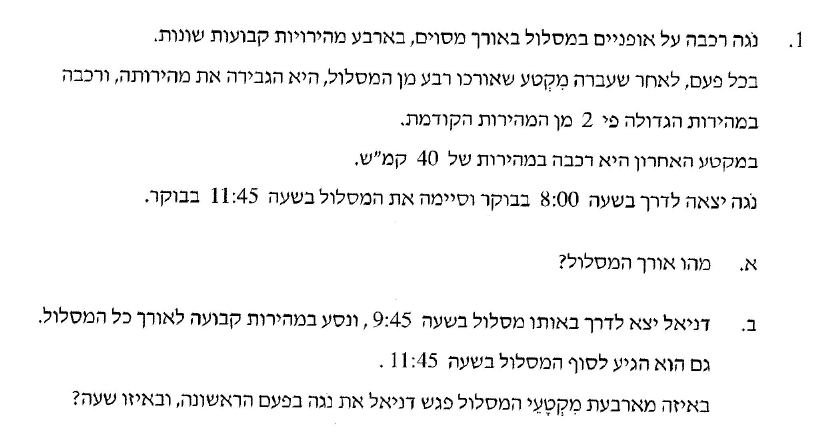
\includegraphics[width=.8\textwidth]{summer-2017a-1}
\end{center}

\begin{center}
\selectlanguage{english}
\begin{tikzpicture}[scale=1]
\draw (0,0) node[below] {\p{08:00}} -- (11.25,0) node[below] {\p{11:45}};
\draw (0,0) -- (0,6);
\draw[thick,name path=noga] (0,0) -- (6,1.5) -- (9,3) -- (10.5,4.5) --  node[right] {
\R{נגה}
} (11.25,6);
\draw[dashed] (0,6) -- +(11.25,0);
\draw[dashed] (0,4.5) -- +(10.5,0);
\draw[dashed] (0,3) -- +(9,0);
\draw[dashed] (0,1.5) -- +(6,0);
\draw[dashed] (6,0) -- (6,1.5);
\draw[dashed] (9,0) -- (9,3);
\draw[dashed] (10.5,0) -- (10.5,4.5);
\draw[dashed] (11.25,0) -- (11.25,6);
\fill (0,0) circle [radius=2pt];
\fill (6,1.5) circle [radius=2pt];
\fill (9,3) circle [radius=2pt];
\fill (10.5,4.5) circle [radius=2pt];
\fill (11.25,6) circle [radius=2pt];
\path (0,0) -- node[left] {$x$} (0,1.5) -- node[left] {$x$} (0,3) -- node[left] {$x$} (0,4.5) -- node[left] {$x$} (0,6);
\draw[thick,name path=dan] (5.25,0) node[below] {\p{09:45}} --  node[left,xshift=16pt,yshift=20pt] {
\R{דניאל}
} (11.25,6);
\path [name intersections={of=noga and dan,by=meeting}];
\draw[dashed] (meeting) |- coordinate (time) (0,0);
\fill (5.25,0) circle [radius=2pt];
\fill (meeting) circle [radius=2pt];
\fill (time) circle [radius=2pt];
\draw[<->] (0,-7mm) -- node[below] {$t_1$} +(6,0);
\draw[<->] (6,-7mm) -- node[below] {$t_2$} +(3,0);
\draw[<->] (6,3mm) -- node[above] {$t$} (time |- 6,3mm);
\draw[<->] (9,-7mm) -- node[below] {$t_3$} +(1.5,0);
\draw[<->] (10.5,-7mm) -- node[below] {$t_4$} +(.75,0);
\end{tikzpicture}
\end{center}

נסמן:
$=x$
המרחק של מקטע,
$=t_1,t_2,t_3,t_4$
זמני רכיבה של נגה במקטעים.

נתון: 
$=40$
המהירות במקטע האחרון, לכן המהירויות של המקטעים האחרים הן
$5,10,20$.

\textbf{סעיף א}

נתון לנו הזמן הכולל והמהירויות )המהירות האחרונה אבל אפשר לחשב את האחרות(, והנעלם היחיד הוא המרחק. נסכם את הזמנים של המקטעים:
\[
\left(\frac{x}{5}+\frac{x}{10}+\frac{x}{20}+\frac{x}{40}\right) = \frac{15}{4}\,.
\]
הפתרון הוא
$x=10$
ולכן אורך המסלול הוא
$40$
ק"מ.

\np

\textbf{סעיף ב}

חישבנו את המרחק ונתון הזמן של דניאל. המהירות של דניאל היא 
$40/2=20$
קמ"ש.

יכול להיות שאפשר למצוא נוסחה עבור המפגש, אבל פשוט יותר לעובר מקטע מקטע ולבדוק אם המפגש מתקיים באותו מקטע.

נגה עוברת
$10$
ק"מ בכל מקטע. מה המרחק שעובר דניאל עד סוף המקטע הראשון?

$t_1 = 10/5 = 2$
כך שסוף המקטע הוא ב- 
\L{\p{10:00}}.
דניאל רוכב רבע שעה מ-
\L{\p{09:45}}
ועד
\L{\p{10:00}}
ולכן המרחק שהוא עובר הוא רק
$\displaystyle 20\cdot\frac{1}{4} = 5$
ק"מ והמפגש לא התקיים במקטע הראשון.


מתי נגה מגיעה לסוף המקטע השני?
$t_2=10/10 =1$
כך שסוף המקטע הוא ב-%
\L{\p{11:00}}.
בשעה ורבע בין 
\L{\p{09:45}}
ל
\L{\p{11:00}}
דניאל רוכב
$\displaystyle 20\cdot \frac{5}{4}=25$
ק"מ, מרחק גדול מהמרחק של נגה, לכן המפגש מתקיים במקטע השני.

\medskip

נשאר רק לחשב את פרק הזמן בתוך המקטע השני עד למפגש, שנסמן
$t$.
נכתוב משוואה למרחקים השווים של נגה ודניאל. נגה רכבה
$10$
ק"מ עד סוף הקטע הראשון ודניאל רכב 
$5$
ק"מ. מסוף הקטע הראשון, הם רכבו 
$t$
שעות, כל אחד במהירות שלו:
\erh{12pt}
\begin{equationarray*}{rcl}
10 + 10t &=& 5 + 20t\\
t&=&\frac{1}{2}\,.
\end{equationarray*}
כבר חישבנו שתחילת המקטע השני בשעה
\L{\p{10:00}},
ולכן שעת המפגש היא
\L{\p{10:30}}.

%%%%%%%%%%%%%%%%%%%%%%%%%%%%%%%%%%%%%%%%%%%%%%%%%%%%%%%%%%%%%%%%

\np

\section{חורף תשע"ז}

\begin{center}
\selectlanguage{english}
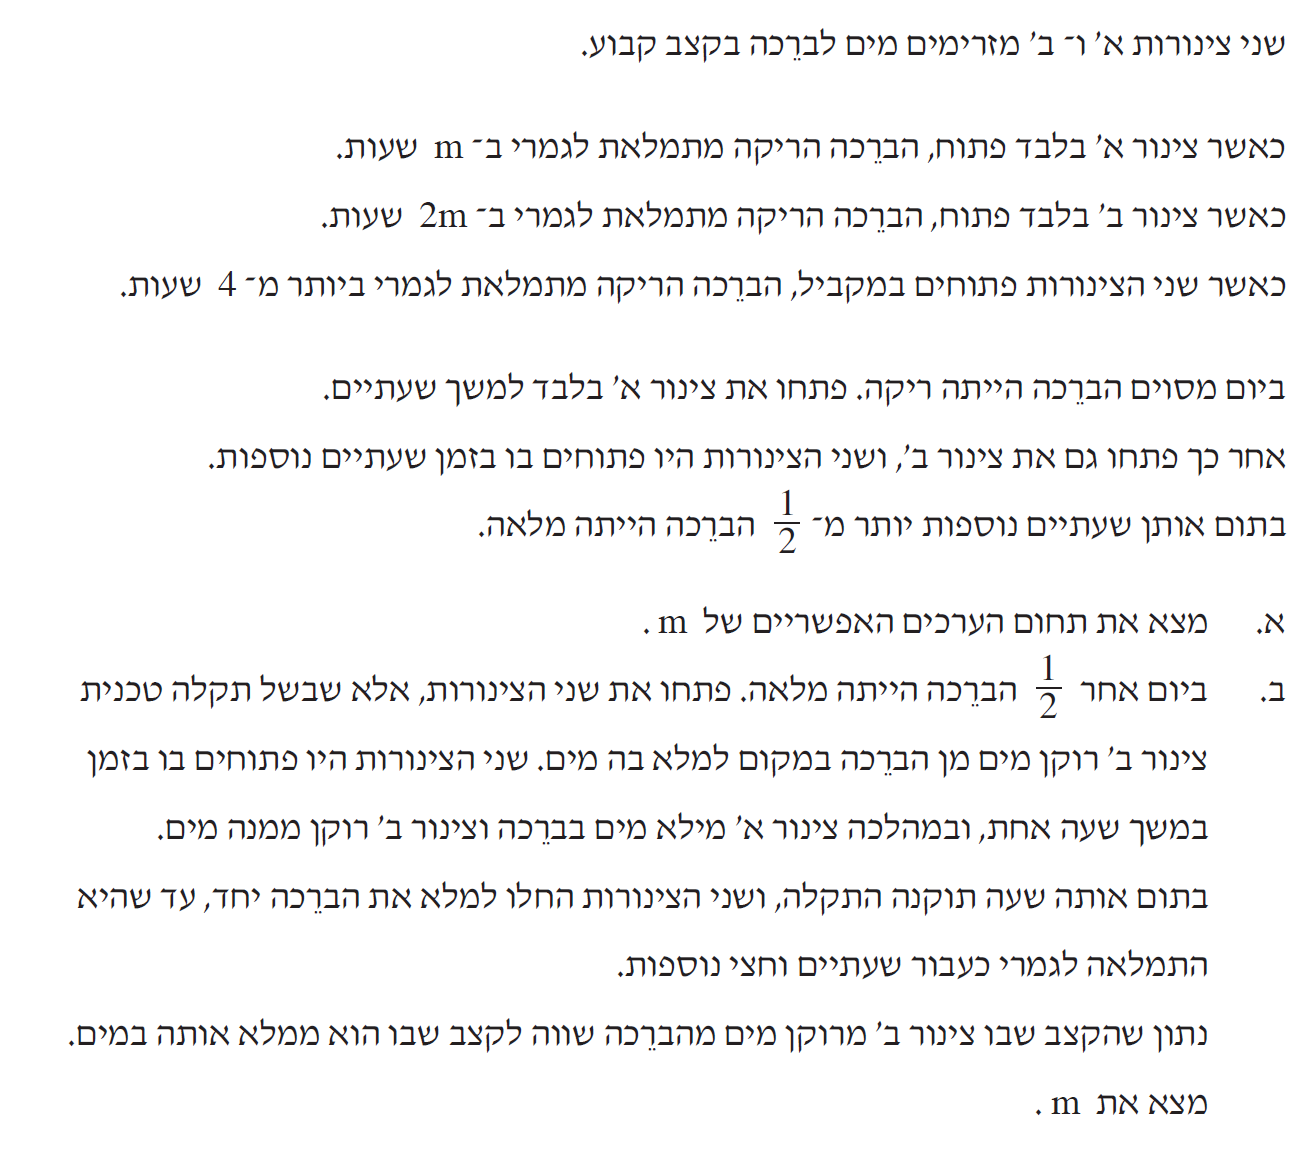
\includegraphics[width=.9\textwidth]{winter-2017-1}
\end{center}

\textbf{סעיף א}

\begin{center}
\selectlanguage{english}
\begin{tikzpicture}[scale=.8]
\draw (0,0) -- (10,0);
\draw (0,0) node[left] {\R{בריכה ריקה}} -- (0,6) node[left] {\R{בריכה מליאה}};
\draw[dashed] (0,6) -- (10,6);
\draw[thick] (0,0) -- node[right,near end,xshift=2mm,yshift=-2mm] {
\R{ב}
} node[right,xshift=12mm,yshift=4mm] {$\displaystyle\frac{1}{2m}$}(9,6);
\draw[thick] (0,0) -- node[left,near end,xshift=-3mm] {
\R{א}
} node[left,xshift=-2mm,yshift=3mm] {$\displaystyle\frac{1}{m}$} (4.5,6);
\draw[dashed] (9,6) -- (9,0);
\draw[dashed] (4.5,6) -- (4.5,0);
\draw[<->] (0,-.6) -- node[fill=white] {$m$} (4.5,-.6);
\draw[<->] (0,-1.2) -- node[fill=white] {$2m$} (9,-1.2);
\end{tikzpicture}
\end{center}
כאשר שני הצינורות פתוחים, ההספק הכולל הוא סכום ההספקים של הצינורות. לפי הנתונים:
\[
1/\left(\frac{1}{m}+\frac{1}{2m}\right) > 4\,,
\]
כך ש-%
$m>6$.

\begin{center}
\selectlanguage{english}
\begin{tikzpicture}
\draw (0,0) -- (10,0);
\draw (0,0) node[left] {\R{בריכה ריקה}}
-- (0,4) node[left] {\R{בריכה מליאה}};
\draw[thick] (4,0) -- node[above,near end,yshift=2mm] {
\R{ב}
} node[above,near start,yshift=2mm] {$\displaystyle\frac{1}{2m}$}(8,1);
\draw[thick] (0,0) -- node[left,near end,xshift=-3mm] {
\R{א}
} node[left,xshift=-2mm,yshift=3mm] {$\displaystyle\frac{1}{m}$} (8,4);
\draw[dashed] (8,4) -- (8,0);
\draw[dashed] (4,2) -- (4,0);
\draw[<->] (0,-.6) -- node[fill=white] {$2$} (4,-.6);
\draw[<->] (0,-1.2) -- node[fill=white] {$4$} (8,-1.2);
\draw[<->] (9,0) -- node[fill=white] {$w_a$} (9,4);
\draw[<->] (8.5,0) -- node[fill=white] {$w_b$} (8.5,1);
\end{tikzpicture}
\end{center}
נסמן:
$=w_a$
כמות המים שמילא צינור א,
$=w_b$
כמות המים שמילא צינור ב.

\smallskip

כמות המים לאחר ארבע שעות שווה לסכום הכמויות שכל צינור מילא והיא לפחות מחצית הבריכה:
\[
w_a + w_b = \frac{1}{m}\cdot 4 + \frac{1}{2m}\cdot 2 > \frac{1}{2}\,.
\]
מכאן,
$m<10$.

\smallskip

\textbf{סעיף ב}

\begin{center}
\selectlanguage{english}
\begin{tikzpicture}[scale=.9]
\draw (0,0) -- (9,0);
\draw (0,0) node[left] {\R{בריכה ריקה}}
-- (0,6) node[left] {\R{בריכה מליאה}};
\draw[dashed] (0,6) -- (9,6);
\draw[thick] (0,3) -- node[below right,xshift=10mm,yshift=-4mm] {$\displaystyle\frac{1}{m}-\frac{1}{2m}=\frac{1}{2m}$} (2,3.5);
\draw[->] (2.2,2.15) -- +(140:1.6cm);
\draw[thick] (2,3.5) -- node[left,xshift=-4mm,yshift=3mm] {$\displaystyle\frac{1}{m}+\frac{1}{2m}=\frac{3}{2m}$} (7,6);
\draw[dashed] (2,3.5) -- (2,0);
\draw[dashed] (2,3.5) -- (0,3.5);
\draw[dashed] (7,6) -- (7,0);
\draw[<->] (0,-.6) -- node[fill=white] {$1$} (2,-.6);
\draw[<->] (2,-1.2) -- node[fill=white] {$2.5$} (7,-1.2);
\node at (-.4,3) {$\displaystyle\frac{1}{2}$};
\end{tikzpicture}
\end{center}
כדי למלא את הבריכה, מתחילים ממחצית הכמות, מוסיפים )מחסירים כי שלילי( את הכמות של השעה הראשונה, ומוסיפים את הכמות מהתקופה השניה של שעתיים וחצי:
\[
\frac{1}{2} + \left(\frac{1}{m}-\frac{1}{2m}\right)\cdot 1 + \left(\frac{1}{m}+\frac{1}{2m}\right)\cdot 2.5 = 1\,.
\]
הפתרון הוא
$m=8.5$.

%%%%%%%%%%%%%%%%%%%%%%%%%%%%%%%%%%%%%%%%%%%%%%%%%%%%%%%%%%%%%%%%

\np

\section{קיץ תשע"ו, מועד ב}

\begin{center}
\selectlanguage{english}
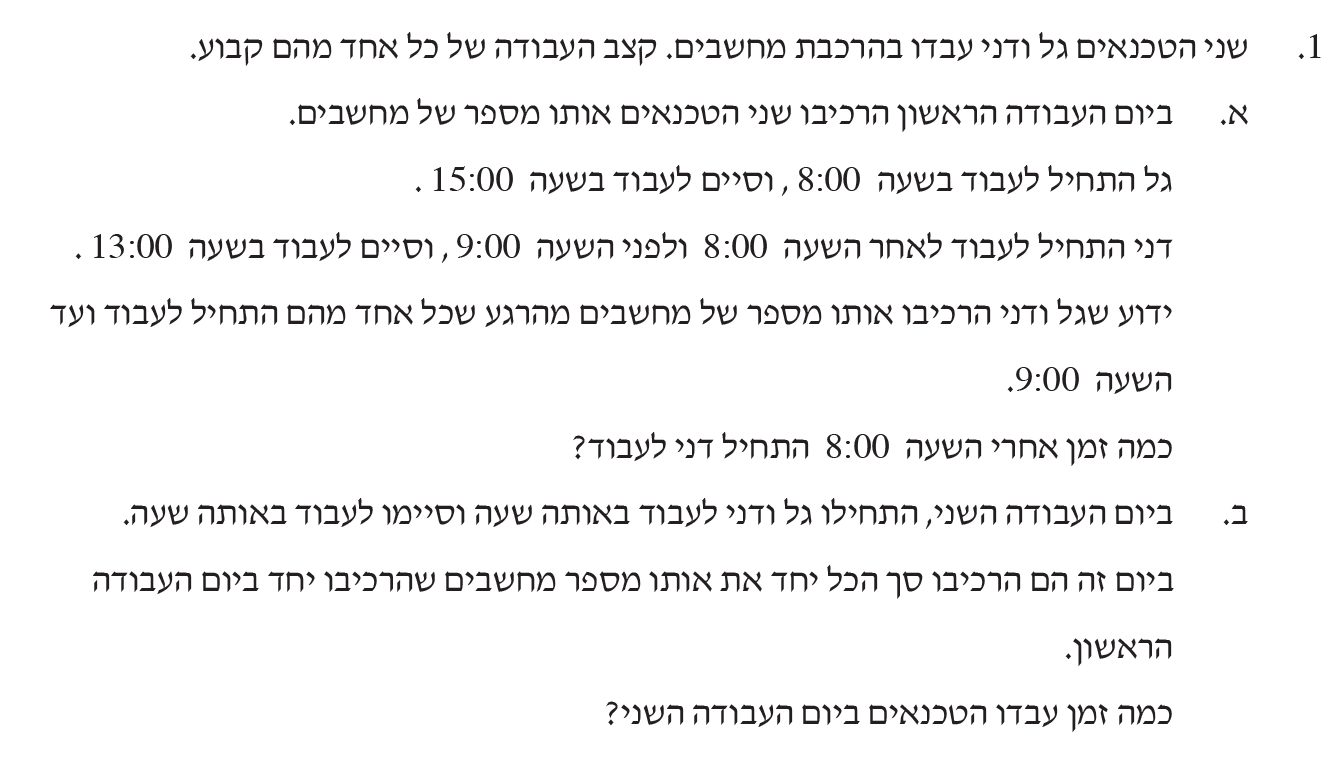
\includegraphics[width=\textwidth]{summer-2016b-1}
\end{center}

\textbf{סעיף א}

\begin{center}
\selectlanguage{english}
\begin{tikzpicture}
\draw (0,0) -- (10,0);
\draw (0,0) node[above left] {\R{אף מחשב לא הורכב}}
-- (0,6) node[left] {\R{כל המחשבים הורכבו}};
\draw[dashed] (0,6) -- (10,6);
\draw[thick,name path=gal] (0,0) -- node[right,near end,xshift=3mm] {
\R{גל}
} node[right,xshift=7mm] {$\displaystyle\frac{1}{7}$}(10,6);
\draw[thick,name path=danny] (1.2,0) -- node[left,near end,xshift=-3mm] {
\R{דני}
} node[left,yshift=3mm] {$\displaystyle\frac{1}{(1-t)+4}$} (7,6);
\draw[dashed] (7,6) -- (7,0);
\draw[dashed] (10,6) -- (10,0);
\path [name intersections={of=gal and danny,by=inter}];
\fill (inter) circle [radius=2pt];
\draw[dashed] (inter) -- (inter |- 0,0);
\draw[dashed] (inter) -- (inter -| 0,0);
\node[below] at (0,0) {\p{08:00}};
\node[below] at (1.2,0) {$t$};
\node[below] at (inter |- 0,0) {\p{09:00}};
\node[below] at (7,0) {\p{13:00}};
\node[below] at (10,0) {\p{15:00}};
\end{tikzpicture}
\end{center}

נסמן:
$=t$
הזמן שדני התחיל בהרכבה.

נשתמש בנתונים כדי למצוא ביטויים עבור ההספקים של דני וגל. נתייחס לסך המחשבים שהרכיב כל אחד כיחידת עבודה אחת. גל עבד שבע שעות ולכן ההספק שלו הוא
$\displaystyle \frac{1}{7}$,
ודני עבד 
$1-t$
עד לשעה 
\L{\p{09:00}}
ואחר כך עוד ארבע שעות. ההספק שלו הוא
$\displaystyle \frac{1}{(1-t)+4}$.

\np
נתון שבשעה 
\L{\p{0900}}
שניהם סיימו להרכיב אותו כמות של מחשבים:
\[
\frac{1}{7}\cdot 1 = \frac{1}{5-t} \cdot (1-t)\,,
\]
ולכן דני התחיל לעבוד
$\displaystyle t=\frac{1}{3}$
שעה לאחר
\L{\p{08:00}}.

\smallskip

\textbf{סעיף ב}

נצייר תרשים חדש עם המידע לסעיף זה.

\begin{center}
\selectlanguage{english}
\begin{tikzpicture}
\draw (0,0) -- (10,0);
\draw (0,0) node[above left] {\R{אף מחשב לא הורכב}}
-- (0,6) node[left] {\R{כל המחשבים הורכבו}};
\draw[dashed] (0,6) -- (10,6);
\draw[thick] (0,0) -- node[right,near end,xshift=2mm,yshift=-2mm] {
\R{גל}
} node[right,xshift=6mm,yshift=-3mm] {$\displaystyle\frac{1}{7}$}(8,2.5);
\draw[thick] (0,0) -- node[left,near end,xshift=-3mm] {
\R{דני}
} node[left,xshift=-2mm,yshift=3mm] {$\displaystyle\frac{3}{14}$} (8,6);
\draw[dashed] (8,6) -- (8,0);
\draw[<->] (0,-.6) -- node[fill=white] {$T$} (8,-.6);
\draw[<->] (8.6,0) -- node[fill=white] {$w_g$} (8.6,2.5);
\draw[<->] (9.2,0) -- node[fill=white] {$w_d$} (9.2,6);
\end{tikzpicture}
\end{center}
נסמן: 
$=T$
הזמן ששניהם עבדו ביום השני. על התרשים סימנו גם את כמות העבודה שעשה כל אחד מהם:
$=w_g$
העבודה של גל,
$=w_d$
העבודה של דני.

\smallskip

בסעיף א הערנו שההספק של גל הוא
$\displaystyle \frac{1}{7}$,
וחישבנו שדני עבד:
\[
\left(1-\frac{1}{3}\right)+4=\frac{14}{3}
\]
שעות. ההספק שלו הוא:
\[
\frac{1}{\frac{14}{3}}=\frac{3}{14}\,.
\]
נתון שהם סיימו אותה כמות עבודה כמו היום הראשון:
\[
1+1=w_g+w_d=\frac{1}{7}T + \frac{3}{14}T\,,
\]
והפתרון הוא 
$T=\displaystyle \frac{28}{5}$.

%%%%%%%%%%%%%%%%%%%%%%%%%%%%%%%%%%%%%%%%%%%%%%%%%%%%%%%%%%%%%%%%

\np

\section{קיץ תשע"ו מועד א}

\begin{center}
\selectlanguage{english}
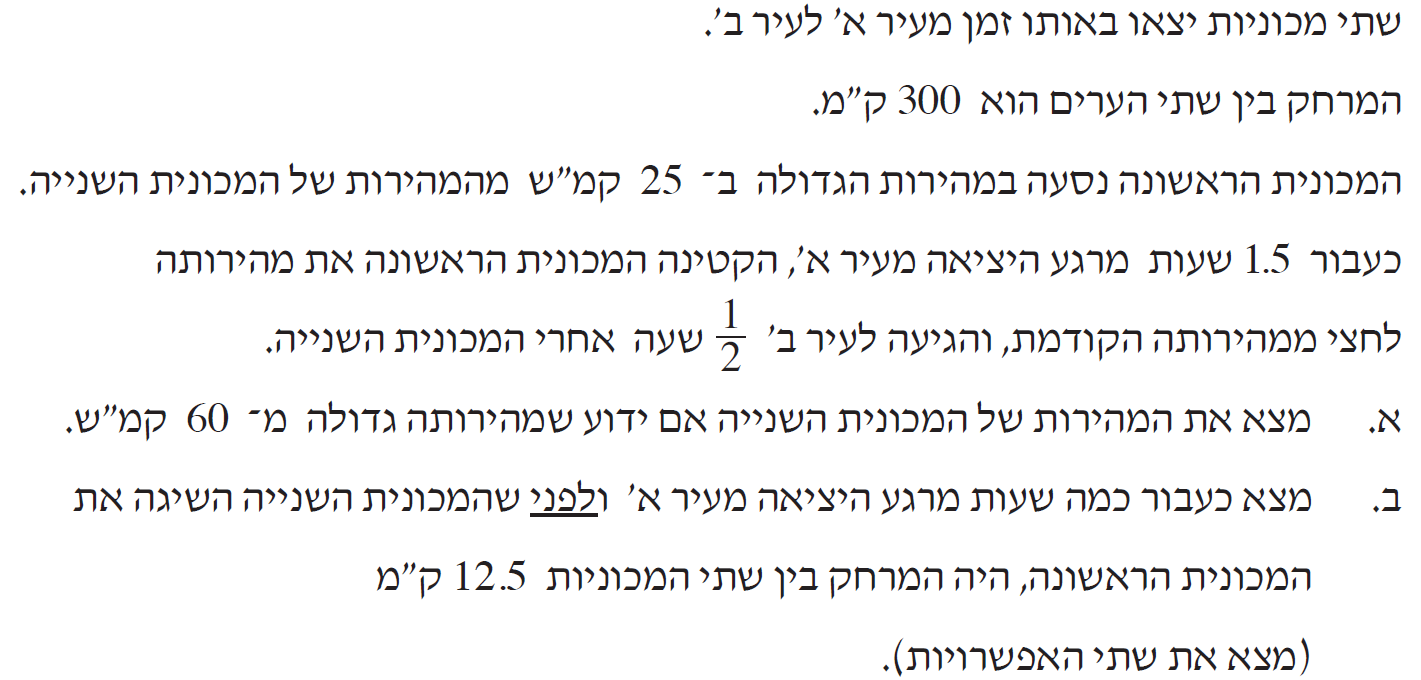
\includegraphics[width=.8\textwidth]{summer-2016a-1}
\end{center}

\begin{center}
\selectlanguage{english}
\begin{tikzpicture}
\draw (0,0) node[left] {
\R{א}
} -- (10,0);
\draw (0,0) -- node[left] {
\R{ק"מ}
$300$} (0,6) node[left] {
\R{ב}
};
\draw[dashed] (0,6) -- (10,6);
\draw[thick,name path=car1] (0,0) -- (3,4) coordinate (change) -- node[above left,near start] {$1$
\R{מכונית}
} (10,6);
\draw[thick,name path=car2] (0,0) -- node[right,xshift=1pt,yshift=-12pt] {$2$
\R{מכונית}
} (7,6);
\draw[dashed] (change) |- coordinate (time) (0,0);
\draw[dashed] (7,6) -- (7,0);
\draw[dashed] (10,6) -- (10,0);
\fill (0,0) circle [radius=2pt];
\fill (7,0) circle [radius=2pt];
\fill (10,0) circle [radius=2pt];
\fill (change) circle [radius=2pt];
\fill (time) circle [radius=2pt];
\draw[<->] (0,-5mm) -- node[fill=white] {
\R{שעות}
$3/2$} (time |- 0,-5mm);
\draw[<->] (7,-5mm) -- node[fill=white] {
\R{שעה}
$1/2$} (10,-5mm);
\draw[<->] (0,-10mm) -- node[fill=white] {$t$} (7,-10mm);
\end{tikzpicture}
\end{center}


נסמן:
$=v_1$
מהירות התחלתית של מכונית
$1$,
$=v_2$
מהירות מכונית
$2$,
$=t$
זמן נסיעה של מכונית
$2$
מעיר א' עד לעיר ב'.

נתון:
$v_1 = v_2+25$.
השיפוע של הקו של מכונית 
$1$
גדולה מהשיפוע של הקו של מכונית 
$2$.

\textbf{סעיף א}

שתי המכוניות נסעו אותו מרחק מעיר א לעיר ב. נכתוב את משוואות התנועה של שתי המכוניות:
\begin{eqnarray*}
v_1\cdot\frac{3}{2} + \frac{v_1}{2}\left(\left(t-\frac{3}{2}\right)+\frac{1}{2}\right) &=& 300\\
v_2t &=& 300\,.
\end{eqnarray*}
נציב 
$v_1 = v_2+25$,
$t = 300/v_2$
במשוואה הראשונה ונקבל משוואה ריבועית ב-%
$v_2$:
\[
v_2^2 - 125v_2 + 3750 = 0\,.
\]
השורשים הם
$50,75$
ונתון ש-%
$v_2>60$
כך שיש לבחור
$v_2=75$
קמ"ש.

\np

\textbf{סעיף ב}

נצייר תרשים חדש עם המידע עבור סעיף זה:

\begin{center}
\selectlanguage{english}
\begin{tikzpicture}
\draw (0,0) node[left] {
\R{א}
} -- (10,0);
\draw (0,0) -- node[left] {
\R{ק"מ}
$300$} (0,6) node[left] {
\R{ב}
};
\draw[dashed] (0,6) -- (10,6);
\draw[thick,name path=car1] (0,0) -- (3,4) coordinate (change) -- node[above left,near start] {$1$
\R{מכונית}
} (10,6);
\draw[thick,name path=car2] (0,0) -- node[right,xshift=32pt,yshift=20pt] {$2$
\R{מכונית}
} (8,6);
\path [name path=time1] (1.2,0) -- (1.2,6);
\path [name path=time2] (5,0) -- (5,6);
\path [name intersections={of=car1 and time1,by=meeting11}];
\path [name intersections={of=car1 and time2,by=meeting12}];
\path [name intersections={of=car2 and time1,by=meeting21}];
\path [name intersections={of=car2 and time2,by=meeting22}];
\draw[thick] (meeting11) -- (meeting21);
\draw[thick] (meeting12) -- (meeting22);
\draw[dashed] (meeting21) |- coordinate (t1) (0,0);
\draw[dashed] (meeting22) |- coordinate (t2) (0,0);
\draw[dashed] (change) |- coordinate (time) (0,0);
\fill (0,0) circle [radius=2pt];
\fill (t1) circle [radius=2pt];
\fill (t2) circle [radius=2pt];
\fill (change) circle [radius=2pt];
\fill (time) circle [radius=2pt];
\draw[<->] (0,-5mm) -- node[fill=white] {$t_1$} (t1 |- 0,-5mm);
\draw[<->] (0,-10mm) -- node[fill=white] {
\R{שעות}
$3/2$} (time |- 0,-10mm);
\draw[<->] (0,-15mm) -- node[fill=white] {$t_2$} (t2 |- 0,-15mm);
\end{tikzpicture}
\end{center}

הקווים האנכיים הכלואים בין הקווים של שתי המכוניות מסמנים מרחק של
$12.5$
ק"מ. קו אחד הוא לפני שינוי המהירות בזמן
$t_1$
מתחילת הנסיעה וקו שני לאחר שינוי המהירות.

בסעיף א' חישבנו
$v_2=75$
ולכן
$v_1=v_2+25=100$.

\smallskip

נכתוב את המשוואות עבור הפרשי המרחקים:
\begin{eqnarray*}
100t_1 - 75t_1 &=& 12.5\\
\left(100\cdot \frac{3}{2} + 50\left(t_2-\frac{3}{2}\right)\right) - 75t_2&=& 12.5\,.
\end{eqnarray*}
הפתרונות הם
$\displaystyle t=\frac{1}{2}, t_2=\frac{5}{2}$
שעות.


%%%%%%%%%%%%%%%%%%%%%%%%%%%%%%%%%%%%%%%%%%%%%%%%%%%%%%%%%%%%%%%%

\np

\section{חורף תשע"ו}

\begin{center}
\selectlanguage{english}
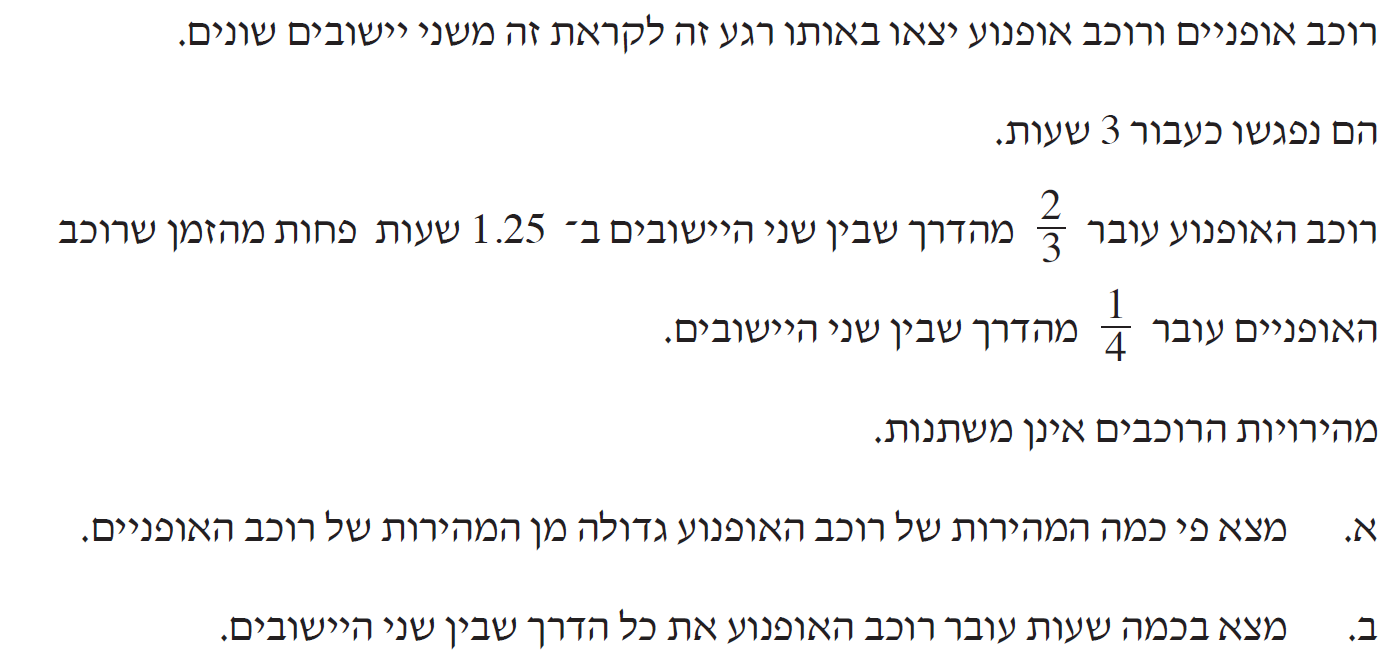
\includegraphics[width=.8\textwidth]{winter-2016-1}
\end{center}

\textbf{סעיף א}

\begin{center}
\selectlanguage{english}
\begin{tikzpicture}
\draw (0,0) node[left] {$A$} -- (10,0);
\draw (0,0) -- (0,6) node[left] {$B$};
\draw[dashed] (0,6) -- (10,6);
\draw[thick,name path=motor] (0,0) -- node[right,near start,xshift=1pt,yshift=-4pt] {
\R{אופנוע}
} (4,6);
\draw[thick,name path=bike] (0,6) -- node[above,near end,xshift=44pt,yshift=-10pt] {
\R{אופניים}
} (8,4);
\node at (8.4,3.7) {$\cdots$};
\path [name intersections={of=motor and bike,by=meeting}];
\coordinate (fourth) at (0,4.5);
\coordinate (two-thirds) at (0,3.5);
\path [name path=path-fourth] (fourth) -- +(6,0);
\path [name path=path-two-thirds] (two-thirds) -- +(6,0);
\path [name intersections={of=path-fourth and bike,by=meeting-fourth}];
\path [name intersections={of=path-two-thirds and motor,by=meeting-two-thirds}];
\draw[dashed] (meeting) |- coordinate (time) (0,0);
\draw[dashed] (meeting-fourth) -| coordinate (fourth-y) (0,0);
\draw[dashed] (meeting-fourth) |- coordinate (fourth-x) (0,0);
\draw[dashed] (meeting-two-thirds) -| coordinate (two-thirds-y) (0,0);
\draw[dashed] (meeting-two-thirds) |- coordinate (two-thirds-x) (0,0);
\fill (meeting) circle [radius=2pt];
\fill (time) circle [radius=2pt];
\fill (0,0) circle [radius=2pt];
\fill (two-thirds) circle [radius=2pt];
\fill (fourth) circle [radius=2pt];
\fill (fourth-x) circle [radius=2pt];
\fill (fourth-y) circle [radius=2pt];
\fill (meeting-fourth) circle [radius=2pt];
\fill (two-thirds-x) circle [radius=2pt];
\fill (two-thirds-y) circle [radius=2pt];
\fill (meeting-two-thirds) circle [radius=2pt];
\path (0,0) -- node[left] {$2/3$} (two-thirds-y);
\path (0,6) -- node[left] {$1/4$} (fourth-y);
\draw[<->] (0,-.5) -- node[fill=white] {
\R{שעות}
 $3$} (time |- 0,-.5);
\draw[<->] (fourth-x |- 0,-1) -- node[fill=white] {
\R{שעות}
$5/4$} (two-thirds-x |- 0,-1);
\node[above left] at (two-thirds-x) {$T_m$};
\node[above right] at (fourth-x) {$T_b$};
\end{tikzpicture}
\end{center}

נסמן:
$=v_b$
מהירות אופניים,
$=v_m$
מהירות אופנוע,
$=x$
מרחק בין הערים,
$=T_m$
פרק הזמן שהאופנוע עובר
$\displaystyle \frac{2}{3}$
מהדרך, פרק הזמן שהאופניים עובר
$\displaystyle \frac{1}{4}$
מהדרך.

כאשר שני כלי רכב היוצאים מנקודות שונות נפגשים, סכום המרחקים שהם עוברים הוא המרחק בין הנקודות. לא נתון המרחק, ולכן אנו משתמשים בנעלם:
\[
x = 3v_b + 3 v_m\,.
\]
הנתון השני הוא הקשר בין זמני הנסיעה של חלקי המרחק בין היישובים:
\[
\frac{x/4}{v_b} = \frac{2x/3}{v_m} + \frac{5}{4}\,.
\]
נסמן את היחס בין המהירויות )התשובה הדרושה(
$r=\frac{v_m}{v_b}$
ונקבל משוואה הריבועית:
\[
3r^2 - 10r - 8 = 0\,.
\]
השורש החיובי הוא
$r=4$.

\np

\textbf{סעיף ב}

נתונה משוואת המרחק בין היישובים:
\[
x = 3v_b + 3 v_m\,.
\]
נשתמש ביחס שחישבנו בסעיף א כדי לחשב את הזמן של נסיעת האופנוע:
\[
\frac{x}{v_m} = \frac{3v_b + 3 v_m}{v_m}=3\frac{v_b}{v_m}+3=3\frac{v_m/4}{v_m}+3=\frac{15}{4}
\]
שעות.

%%%%%%%%%%%%%%%%%%%%%%%%%%%%%%%%%%%%%%%%%%%%%%%%%%%%%%%%%%%%%%%%

\np

\section{קיץ תשע"ה מועד ב}

\begin{center}
\selectlanguage{english}
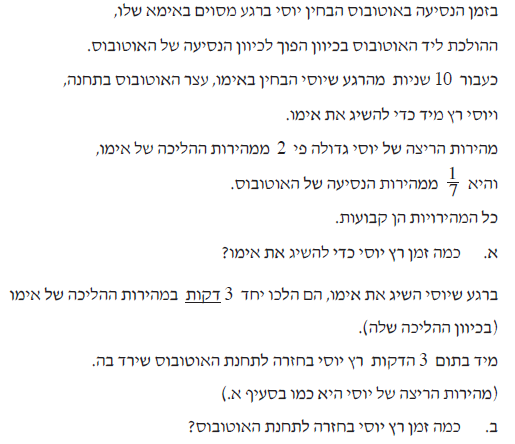
\includegraphics[width=.8\textwidth]{summer-2015b-1}
\end{center}

\vspace{-3ex}

\begin{center}
\selectlanguage{english}
\begin{tikzpicture}[scale=.85]
\draw (0,0) -- (14,0);
\draw (0,-4) node[left] {
\R{פרידה}
} -- (0,-2) node[left] {
\R{מפגש 2}
} -- (0,0) node[left] {
\R{מפגש 1}
} -- (0,4) node[left] {
\R{תחנה}
};
\fill (0,0) circle [radius=2pt];
\fill (1,0) circle [radius=2pt] node[below right] {$M$};
\fill (4,0) circle [radius=2pt] node[above] {$N$};
\fill (8,0) circle [radius=2pt] node[above] {$P$};
\fill (11,0) circle [radius=2pt] node[below right] {$Q$};
\fill (14,0) circle [radius=2pt] node[below] {$R$};
\draw[thick] (0,0) -- node[left] {$a$} (1,4) -- node[right,near start] {$b$} (4,-2);
\draw[thick] (0,0) -- node[below,near start,xshift=-2mm] {$c$} node[right,near end,yshift=2mm] {$d$} (8,-4)  node[below] {$P'$} -- (14,4)  node[right] {$R'$};
\draw[dashed] (0,4) -- (14,4);
\draw[dashed] (0,-2) -- (14,-2);
\draw[dashed] (0,-4) -- (14,-4);
\draw[dashed] (1,4)  node[above] {$M'$} -- (1,0);
\draw[dashed] (4,0) -- (4,-2) node[below,yshift=-1mm] {$N'$};
\draw[dashed] (8,-4) -- (8,0);
\draw[dashed] (11,0) -- (11,4);
\draw[dashed] (14,0) -- (14,4);
\draw[<->] (0,.7) -- node[fill=white] {$10$} (1,.7);
\draw[<->] (1,.7) -- node[near start,fill=white] {$t$} (4,.7);
\draw[<->] (4,.7) -- node[fill=white] {$180$} (8,.7);
\draw[<->] (8,.7) -- node[fill=white] {$t_1$} (11,.7);
\draw[<->] (11,.7) -- node[fill=white] {$t_2$} (14,.7);
\path (8,-2) --  node[below right,xshift=5mm,yshift=-2mm] {$e_1$} (11,0);
\path (11,0) --  node[left,yshift=3mm] {$e_2$} (14,4);
\end{tikzpicture}
\end{center}

\vspace{-3ex}

בתרשים סימנו את הקטעים:
\begin{center}
\begin{tabular}{rr}
\R{$=b$
יוסי רץ לפגישה עם אמא}
&
\R{$=a$
יוסי נוסע באוטובוס}\\
\R{$=d$
יוסי ואמא הולכים ביחד}
&
\R{$=c$
אמא הולכת עד למפגש עם יוסי}\\
&
\R{$=e_1+e_2$
יוסי רץ חזרה לתחנה}
\end{tabular}
\end{center}

\np

נסמן זמן:
$=t$
הזמן שיוסי רץ מהתחנה כדי להשיג את אמא.

נסמן מהירויות:
$=v_y$
יוסי, 
$=v_a$
אמא, 
$=v_b$
אוטובוס.

נתון:
$v_y=2v_a$, $v_y=v_b/7$.

\medskip

\textbf{סעיף א}

מצאתי שקשה לפתור את השאלה עד שציירתי את התרשים המופיע למעלה. את הזמן
$t$
נוכל לחשב ממשוואות התנועה מהמפגש הראשון )יוסי רואה את אימו( ועד למפגש השני )יוסי משיג את אימו(. המרחק מסומן מהתרשים רואים שהמרחק
$NN'$
בתרשים. נוכל למצוא שתי משוואות עבור מרחק זה, אחד עבור אמא, קטע
$c$:
\[
v_a(t+10),
\]
ואחד עבור יוסי, קטעים
$a,b$:
\[
-10v_b + tv_y\,.
\]
שימו לב שבקטע 
$a$
יוסי 
\textbf{מתרחק}
מהמפגש ולכן המרחק הוא שלילי.

יש לנו שני ביטויים עבור אותו מרחק ולאחר הצבת יחסי המהירויות הנתונים נקבל את המשוואה:
\[
\frac{v_y}{2}(t+10) = v_yt - 7v_y 10
\]
שהפתרון שלה הוא
$150=t$
שניות.
\medskip

\textbf{סעיף ב}

מהתרשים קל לראות
\textbf{ששני}
קטעי הקווים
$e_1,e_2$
מתארים את הריצה של יוסי בחזרה לתחנה. רואים גם שהמרחק
$PP'$
של
$e_1$
הוא גם המרחק שאמא הולכת, קטעים 
$c,d$.
לפי התוצאה של סעיף א, לוקח לאמא
$10+150+180=340$
שניות לעבור מרחק זה. נתון שיוסי רץ פי שניים מהר יותר מההליכה של אמא, ולכן
$t_1=170$
שניות.

עבור הקטע השני
$e_2$,
המרחק
$RR'$
שווה למרחק
$MM'$,
המרחק שהאוטובוס עבר מהמפגש הראשון ועד התחנה. נתון שהאוטובוס עובר מרחק זה ב-%
$10$
שניות, ונתון שמהירות הריצה של יוסי פי שבע לאט ממהירות הנסיעה של האוטובוס, כך ש-%
$t_2=70$.

נסכם ונקבל שיוסי רץ מנקודת הפרידה לתחנה ב
$240=t_1+t_2$
שניות.

\textbf{הערה}

שאלה זו שיכנע אותי שתרשים דו-ממיד זמן-מרחק חיוני בפתרון בעיות תנועה.

שימו לב למלכודת: זמן ההליכה היחד נתון בדקות ושאר הזמנים בשניות. אמנם המילה "דקות" מודגש אבל אפשר להתבלבל.

%%%%%%%%%%%%%%%%%%%%%%%%%%%%%%%%%%%%%%%%%%%%%%%%%%%%%%%%%%%%%%%%

\np

\section{קיץ תשע"ה מועד א}

\begin{center}
\selectlanguage{english}
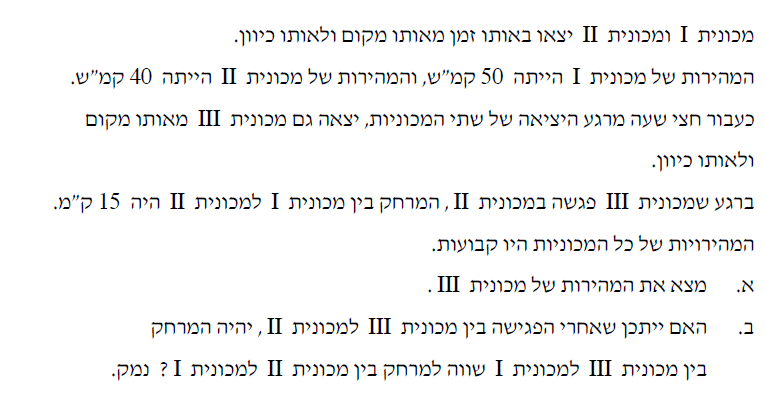
\includegraphics[width=.8\textwidth]{summer-2015a-1}
\end{center}

\begin{center}
\selectlanguage{english}
\begin{tikzpicture}
\draw (0,0) -- (10,0);
\draw (0,0) -- (0,6);
\draw[thick,name path=one] (0,0) -- node[below,near end,xshift=50pt,yshift=28pt] {I} (10,6);
\draw[thick,name path=two] (0,0) -- node[below,near end,xshift=50pt,yshift=14pt] {II} (10,3);
\draw[thick,name path=three] (3,0) -- node[above,near end,xshift=2pt,yshift=12pt] {III} (8,6);
\path [name intersections={of=one and three,by=one-three}];
\path [name intersections={of=two and three,by=two-three}];
\draw[dashed] (two-three) |- coordinate (time-two-three) (0,0);
\fill (0,0) circle [radius=2pt];
\fill (3,0) circle [radius=2pt];
\fill (one-three) circle [radius=2pt];
\fill (two-three) circle [radius=2pt];
\fill (time-two-three) circle [radius=2pt];
\node[above left] at (one-three) {$B$};
\node[below right] at (two-three) {$A$};
\path [name path=distance] (two-three) -| +(0,2);
\path [name intersections={of=one and distance,by=fifteen}];
\draw (two-three) -- (fifteen) node[above left] {
\R{ק"מ}
$15$};
\draw[->] (3.3,2.5) -- (3.8,1.7);
\fill (fifteen) circle [radius=2pt];
\draw[<->] (0,-.6) -- node[fill=white] {
\R{שעה}
 $1/2$} (3,-.6);
\draw[<->] (3,-.6) -- node[fill=white] {$t$} (time-two-three |- 0,-.6);
\end{tikzpicture}
\end{center}
המהירות של מכונית I גדולה מהמהירות של מכונית II, ולכן השיפוע שלו תלול יותר.

נסמן
$=t$
הזמן בין היציאה של III ועד למפגש שלו עם II,
$=v_3$
המהירות של III.

נתון מהירות של I
$v_1=50$,
המהירות של II
$v_2=40$.

\textbf{סעיף א}

לאחר 
$t+1/2$
שעות, המכוניות II ו-III עברו אותו מרחק, ומכונית I עבר אותו מרחק ועוד 
$15$
ק"מ. נכתוב את משוואות התנועה לשני המקרים:
\begin{eqnarray*}
40(t+1/2) &=& v_3t\\
50(t+1/2) &=& v_3t + 15\,.
\end{eqnarray*}
מהמשוואות מתקבל
$t=1$
ואח"כ
$v_3=60$
קמ"ש.

\np

\textbf{סעיף ב}

נוסיף סימונים לתרשים שיעזרו לנו לפתור את הבעייה:

\begin{center}
\selectlanguage{english}
\begin{tikzpicture}
\draw (0,0) -- (10,0);
\draw (0,0) -- (0,6);
\draw[thick,name path=one] (0,0) -- node[below,near end,xshift=50pt,yshift=28pt] {I} (10,6);
\draw[thick,name path=two] (0,0) -- node[below,near end,xshift=50pt,yshift=14pt] {II} (10,3);
\draw[thick,name path=three] (3,0) -- node[above,near end,xshift=2pt,yshift=12pt] {III} (8,6);
\path [name intersections={of=one and three,by=one-three}];
\path [name intersections={of=two and three,by=two-three}];
\draw[dashed] (two-three) |- coordinate (time-two-three) (0,0);
\fill (0,0) circle [radius=2pt];
\fill (3,0) circle [radius=2pt];
\fill (one-three) circle [radius=2pt];
\fill (two-three) circle [radius=2pt];
\fill (time-two-three) circle [radius=2pt];
\node[above left] at (one-three) {$B$};
\node[below right] at (two-three) {$A$};
\path [name path=distance] (two-three) -| +(0,2);
\path [name intersections={of=one and distance,by=fifteen}];
\draw (two-three) -- (fifteen) node[above left] {
\R{ק"מ}
$15$};
\draw[->] (3.3,2.5) -- (3.8,1.7);
\fill (fifteen) circle [radius=2pt];
\draw[<->] (0,-.6) -- node[fill=white] {
\R{שעה}
 $1/2$} (3,-.6);
\draw[<->] (3,-.6) -- node[fill=white] {$t$} (time-two-three |- 0,-.6);
\draw[->] (4.5,3.2) -- +(.45,-.55);
\draw[<->,thick,densely dotted] (5.3,3.1) -- +(0,-1.5);
\draw[<->,thick,densely dotted] (5,2.95) -- +(0,-.5);
\node at (5.6,2.4) {\p{I--II}};
\node at (4.5,3.4) {\p{I--III}};
\draw[<->,thick,densely dotted] (7.8,4.6) -- node[right] {\p{I--II}} +(0,-2.2);
\draw[<->,thick,densely dotted] (7.8,4.8) -- node[right,yshift=3pt] {\p{I--III}} +(0,.8);
\node at (5.6,2.4) {\p{I--II}};
\node at (4.5,3.4) {\p{I--III}};
\end{tikzpicture}
\end{center}

נעיין בקווים מנוקדים בתרשים ונראה שהמרחקים לא יכולים שווים. בנקודה
$A$
הרחקים שווים, אבל מנקודה זו ועד לנקודה
$B$,
המרחק 
\p{I--II}
גדל והמרחק
\p{I--III}
קטן.

בנקודה
$B$
המרחק 
\p{I--II}
חיובי והמרחק
\p{I--III}
שווה לאפס. מכאן והלאה, שני המרחקים גדלים באותו קצב כי הפרשי המהירויות שווים
$10$
קמ"ש.

\smallskip

\textbf{הוכחה בחישוב}

נסמן
$=t_A$
זמן מנקודה
$A$,
$=t_B$
זמן מנקודה
$B$,
$=d_B$
המרחק בין
\p{I}
ל-
\p{II}
בנקודה
$B$.

\smallskip

משמאל לנקודה
$B$
המרחקים שווים
\textbf{אם}:
\[
15 + (v_1-v_2)t_A \stackrel{?}{=} 15 + (v_1-v_3)t_A\,.
\]
נציב
$v_1=50, v_2=40, v_3=60$
ונקבל
$10=-10$,
כך הטיעון לא יכול להיות נכון.

\smallskip

מימין לנקודה
$B$
המרחקים שווים
\textbf{אם}:
\[
(v_3-v_1)t_B \stackrel{?}{=} d_B + (v_1-v_2)t_B\,.
\]
לאחר הצבה עבור המהירויות, נקבל שהטיעון נכון אם
$d_B=0$,
אבל אנחנו יודעים ש-%
$d_B > 15$.

%%%%%%%%%%%%%%%%%%%%%%%%%%%%%%%%%%%%%%%%%%%%%%%%%%%%%%%%%%%%%%%%

\np

\section{חורף תשע"ה}

\begin{center}
\selectlanguage{english}
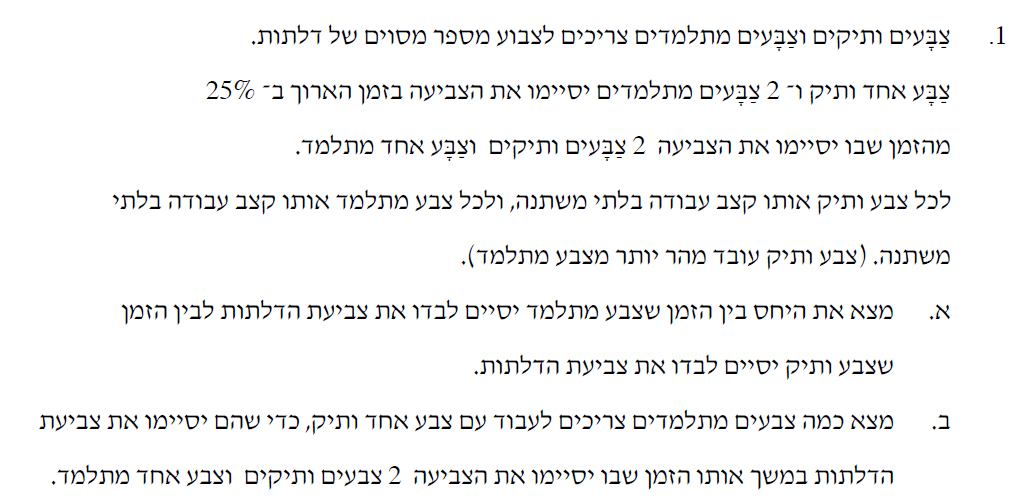
\includegraphics[width=\textwidth]{winter-2015-1}
\end{center}

\vspace{-2ex}

\textbf{סעיף א}

\begin{center}
\selectlanguage{english}
\begin{tikzpicture}
\draw (0,0) -- (10,0);
\draw (0,0) node[above left] {\R{אף דלת לא נצבע}}
-- (0,6) node[left] {\R{כל הדלתות נצבעו}};
\draw[dashed] (0,6) -- (10,6);
\draw[ultra thick] (0,0) -- node[left,near end,xshift=-2mm] {$2/t_v$} (8,4.5)  coordinate (two-one);
\draw[ultra thick] (0,4.5)  -- node[left,xshift=-2mm,yshift=2mm] {$1/t_m$} (8,6) coordinate (two-one-finish);
\draw[dotted,ultra thick] (0,4.5) -- (8,4.5);
\draw[thick] (0,0) -- node[left,yshift=2mm] {$1/t_v$} (10,2.25)  coordinate (one-two);
\draw[thick] (0,2.25)  -- node[left,near start,yshift=2mm] {$2/t_m$} (10,6) coordinate (one-two-finish);
\draw[dotted,thick] (0,2.25) -- (10,2.25);
\draw[dashed] (two-one-finish) -- (two-one-finish |- 0,0);
\draw[dashed] (one-two-finish) -- (one-two-finish |- 0,0);
\draw[<->] (0,-.6) -- node[fill=white] {$T$} (two-one-finish |- 0,-.6);
\draw[<->] (0,-1.2) -- node[fill=white] {$1.25 T$} (one-two-finish |- 0,-1.2);
\end{tikzpicture}
\end{center}
\vspace{-1ex}

נסמן את הזמנים לצביעת כל הדלתות. 
$=t_v$
הזמן שלוקח צבע ותיק,
$=t_m$
הזמן שלוקח צבע מתלמד,
$=T$
הזמן שלוקח שני צבעים ותיקים וצבע מתלמד אחד. למעשה, הערך של
$T$
לא חשוב ואפשר להשתמש ב-%
$1$
כיחידת זמן.

\smallskip

\noindent\textbf{הסבר על התרשים}

הצבעים עובדים במקביל אבל הציר בתרשים מראה
\textbf{חלוקת העבודה},
כאילו שצבע )או זוג צבעים( מסיים את חלקו בעבודה ואחר כך הצבע )או הזוג( השני מתחיל את חלקו. ההספקים מתקבלים מעבודה חלקי זמן. כאשר יש זוג צבעים הם רשומים כצבע אחד עם הספק כפול. הקווים הדקים מראים צבע אחד ותיק 
$(1/t_v)$
ושני צבעים מתלמדים
$(2/t_m)$.
הקווים העבים מראים שני צבעים ותיקים
$(2/t_v)$
וצבע אחד מתלמד
$(1/t_m)$.

\np

שני ההרכבים סיימו את העבודה ומכאן שמשוואת ההספק נותנת אותו ערך עבור שני ההרכבים. )זיכרו שקבענו שהזמנים הם 
$1$
ו-%
$1.25$
עבור שני ההרכבים.(:
\[
\frac{2}{t_v}\cdot 1 \:+\: \frac{1}{t_m}\cdot 1 \;=\; \frac{1}{t_v}\cdot 1.25 \:+\: \frac{2}{t_m} \cdot 1.25 \,.
\]
הפתרון הוא:
\[
\frac{t_m}{t_v}=2\,.
\]

\textbf{סעיף ב}

\begin{center}
\selectlanguage{english}
\begin{tikzpicture}
\draw (0,0) -- (10,0);
\draw (0,0) node[above left] {\R{אף דלת לא נצבע}}
-- (0,6) node[left] {\R{כל הדלתות נצבעו}};
\draw[dashed] (0,6) -- (10,6);
\draw[ultra thick] (0,0) -- node[left,near end,xshift=-2mm] {$2/t_v$} (8,4.5)  coordinate (two-one);
\draw[ultra thick] (0,4.5)  -- node[left,xshift=-2mm,yshift=2mm] {$1/t_m$} (8,6) coordinate (two-one-finish);
\draw[dashed,ultra thick] (0,4.5) -- (8,4.5);
\draw[thick] (0,0) -- node[left,yshift=2mm] {$1/t_v$} (8,2.25)  coordinate (one-two);
\draw[thick] (0,2.25)  -- node[left,near start,yshift=2mm] {$n/t_m$} (8,6) coordinate (one-two-finish);
\draw[dashed,blue] (0,2.25) -- (8,2.25);
\draw[dashed] (two-one-finish) -- (two-one-finish |- 0,0);
\draw[<->] (0,-.6) -- node[fill=white] {$1$} (two-one-finish |- 0,-.6);
\end{tikzpicture}
\end{center}

נסמן
$=n$
מספר הבצעים המתלמדים. העבודה של שני ההרכבים שווה ולכן:
\[
\frac{2}{t_v} + \frac{1}{t_m} = \frac{1}{t_v} + \frac{n}{t_m}\,.
\]
נשתמש ביחס שחישבנו בסעיף א ונקבל:
\[
n = \frac{t_m}{t_v} + \frac{t_m}{t_m} = 2+1=3\,.
\]

%%%%%%%%%%%%%%%%%%%%%%%%%%%%%%%%%%%%%%%%%%%%%%%%%%%%%%%%%%%%%%%%

\np

\section{קיץ תשע"ד מועד ב}

\begin{center}
\selectlanguage{english}
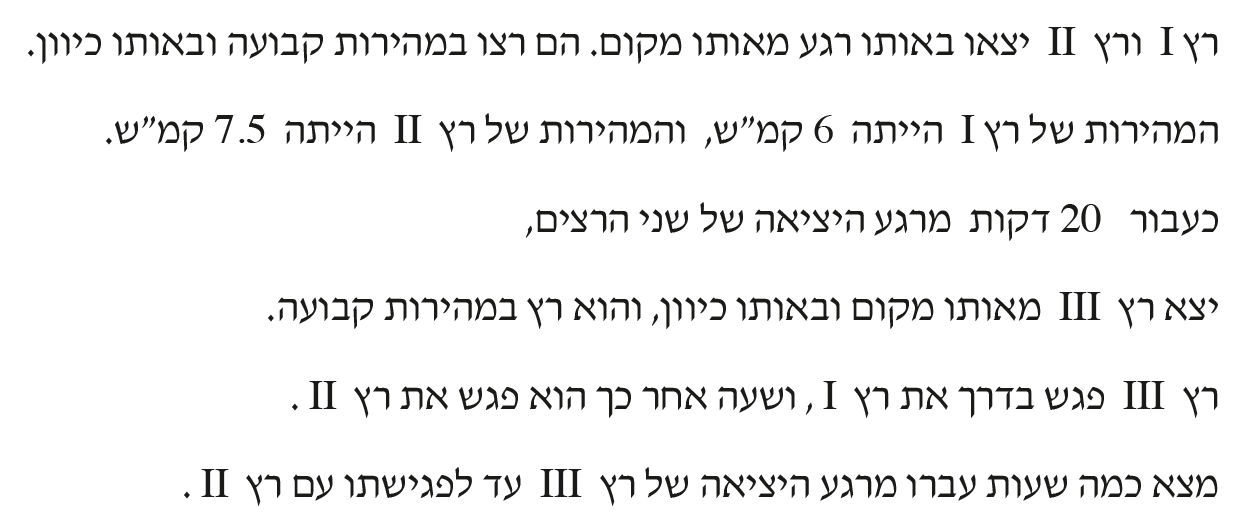
\includegraphics[width=.8\textwidth]{summer-2014b-1}
\end{center}

\begin{center}
\selectlanguage{english}
\begin{tikzpicture}
\draw (0,0) -- (10,0);
\draw (0,0) -- (0,6);
\draw[thick,name path=one] (0,0) -- node[below,near end,xshift=4pt] {I} (10,4);
\draw[thick,name path=two] (0,0) -- node[below,near end,xshift=16pt,yshift=6pt] {II} (10,6);
\draw[thick,name path=three] (2,0) -- node[above,near end,yshift=6pt] {III} (9,6);
\path [name intersections={of=one and three,by=one-three}];
\path [name intersections={of=two and three,by=two-three}];
\draw[dashed] (one-three) |- coordinate (time-one-three) (0,0);
\draw[dashed] (two-three) |- coordinate (time-two-three) (0,0);
\fill (0,0) circle [radius=2pt];
\fill (2,0) circle [radius=2pt];
\fill (one-three) circle [radius=2pt];
\fill (two-three) circle [radius=2pt];
\fill (time-one-three) circle [radius=2pt];
\fill (time-two-three) circle [radius=2pt];
\draw[<->] (0,-.6) -- node[fill=white] {
\R{שעה}
 $1/3$} (2,-.6);
\draw[<->] (2,-.6) -- node[fill=white] {$t$} (time-one-three |- 0,-.6);
\draw[<->] (time-one-three |- 0,-.6) -- node[fill=white] {
\R{שעה}
 $1$} (time-two-three |- 0,-.6);
\end{tikzpicture}
\end{center}

נסמן:
$=t$
הזמן בין היציאה של III ועד למפגש שלו עם I,
$=v$
המהירות של III.

נתון:
$=6$
מהירות של I ו-
$=7.5$
המהירות של II. שימו לב לשיפועים של הקווים.

בכל מפגש בין שתי דמויות המרחקים שווים. המפגש בין I ל-III:
\[
6(t+1/3) = vt\,,
\]
והמפגש בין II ו-III:
\[
7.5(1/3+t+1) = v(t+1)\,.
\]
מהמשוואה הראשונה נקבל ביטוי עבור 
$v$
ונציב במשוואה השנייה. נקבל משוואה ריבועית ב-%
$t$:
\[
1.5t^2 + 2t - 2 = 0\,,
\]
שיש לה פתרון חיובי אחד
$t=2/3$.

\smallskip

הזמן מהיציאה של III ועד המפגש שלו עם II הוא
$t+1=5/3$
שעות.

%%%%%%%%%%%%%%%%%%%%%%%%%%%%%%%%%%%%%%%%%%%%%%%%%%%%%%%%%%%%%%%%

\np

\section{קיץ תשע"ד מועד א}

\begin{center}
\selectlanguage{english}
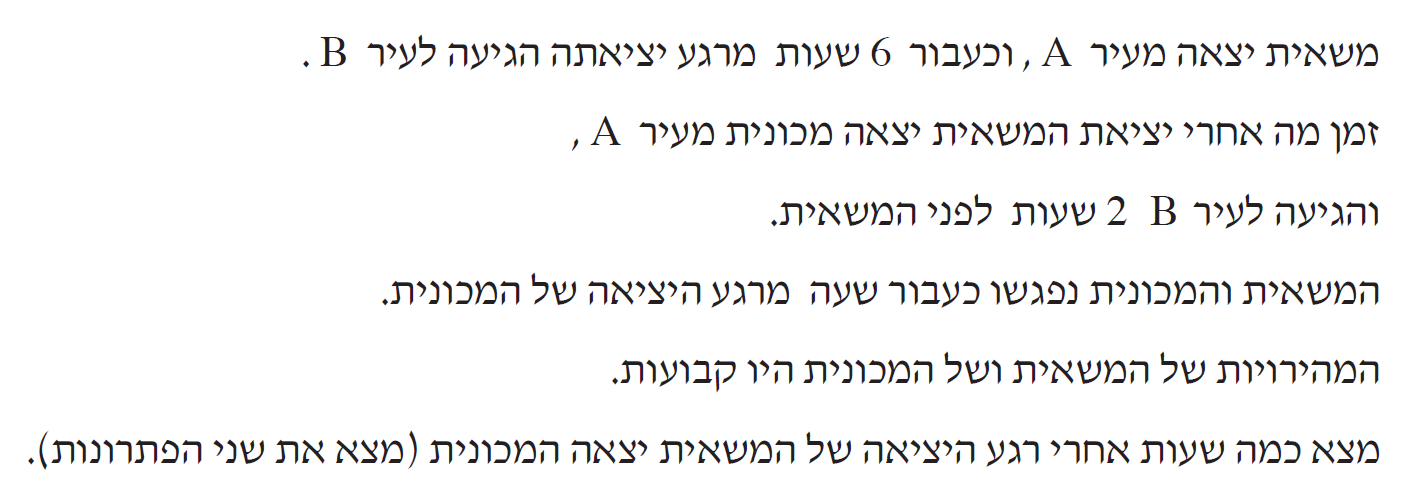
\includegraphics[width=.8\textwidth]{summer-2014a-1}
\end{center}

\begin{center}
\selectlanguage{english}
\begin{tikzpicture}
\draw (0,0) node[left] {$A$} -- (10,0);
\draw (0,0) -- (0,6) node[left] {$B$};
\draw[dashed] (0,6) -- (10,6);
\draw[thick,name path=truck] (0,0) -- node[left,near start,xshift=-6pt] {
\R{משאית}
} (10,6);
\draw[thick,name path=car] (3,0) -- node[left,near end] {
\R{מכונית}
} (7,6);
\path [name intersections={of=truck and car,by=meeting}];
\draw[dashed] (meeting) |- coordinate (time) (0,0);
\draw[dashed] (10,0) -- (10,6);
\draw[dashed] (7,0) -- (7,6);
\fill (meeting) circle [radius=2pt];
\fill (time) circle [radius=2pt];
\fill (0,0) circle [radius=2pt];
\fill (3,0) circle [radius=2pt];
\fill (7,0) circle [radius=2pt];
\fill (10,0) circle [radius=2pt];
\draw[<->] (0,-.5) -- node[fill=white] {$t$} (3,-.5);
\draw[<->] (3,-.5) -- node[fill=white] {
\R{שעה}
 $1$} (time |- 0,-.5);
\draw[<->] (time |- 0,-.5) -- node[fill=white] {$3-t$} (7,-.5);
\draw[<->] (7,-.5) -- node[fill=white] {
\R{שעות}
 $2$} (10,-.5);
\draw[<->] (3.1,-1.2) -- node[fill=white] {$4-t$} (6.9,-1.2);
\draw[<->] (0,-1.8) -- node[fill=white] {
\R{שעות}
 $6$} (10,-1.8);
\end{tikzpicture}
\end{center}

בתרשים חשוב לרשום את כל פרק זמן, במיוחד כדי לקבל את זמן הנסיעה של המכונית.

נסמן:
$=t$
זמן יציאת המכונית,
$=v_c$
מהירות המכונית,
$=v_m$
מהירות המשאית.

\smallskip

נכתוב משוואות למרחקים שווים, מ-
$A$
עד למפגש ומ-
$A$
עד ל-
$B$:
\begin{eqnarray*}
v_m(t+1) &=& v_c\cdot 1\\
v_m \cdot 6 &=& v_c (4-t)\,.
\end{eqnarray*}
משתי המשוואות מתקבלת משוואה ריבועית ב-
$t$:
\[
t^2 - 3t + 2 = 0
\]
שיש לה שני פתרונות
$t=1$
שעה ו-
$t=2$
שעות.

%%%%%%%%%%%%%%%%%%%%%%%%%%%%%%%%%%%%%%%%%%%%%%%%%%%%%%%%%%%%%%%%

\np

\section{חורף תשע"ד}

\begin{center}
\selectlanguage{english}
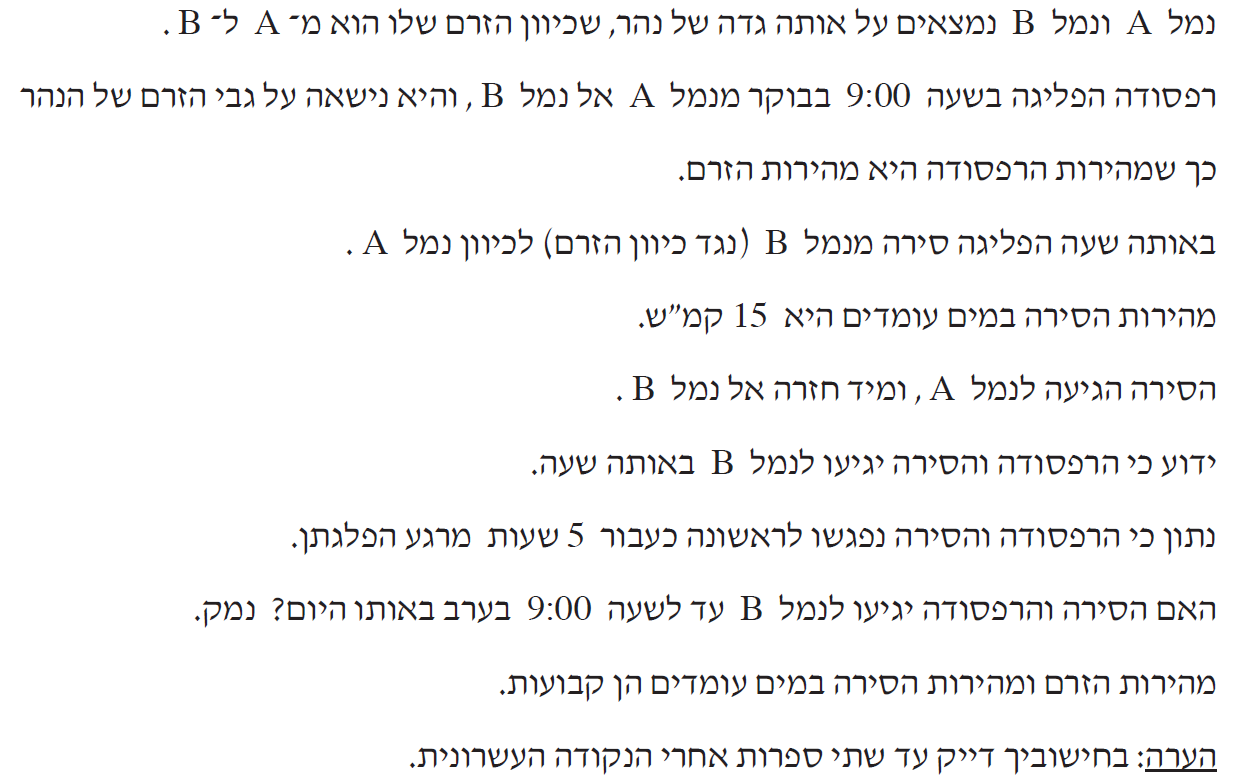
\includegraphics[width=.8\textwidth]{winter-2014-1}
\end{center}

\begin{center}
\selectlanguage{english}
\begin{tikzpicture}
\draw (0,0) node[below left] {$A$} node[below,xshift=-14pt,yshift=-10pt] {\p{9:00}} -- (10,0);
\draw (0,0) -- (0,6) node[above left] {$B$};
\draw[dashed] (0,6) -- (10,6);
\draw[thick,name path=raft] (0,0) -- node[left,near start,xshift=-4pt] {
\R{רפסודה}
} (10,6);
\draw[thick,name path=boat] (0,6) -- node[right,near start,xshift=2pt] {
\R{סירה}
} (8,0) -- (10,6);
\path [name intersections={of=boat and raft,by=meeting}];
\draw[dashed] (meeting) |- coordinate (time) (0,0);
\draw[dashed] (meeting) -| coordinate (distance) (0,0);
\draw[dashed] (8,0) -- (8,6);
\draw[dashed] (10,0) -- (10,6);
\fill (meeting) circle [radius=2pt];
\fill (time) circle [radius=2pt];
\fill (0,0) circle [radius=2pt];
\fill (8,0) circle [radius=2pt];
\fill (8,6) circle [radius=2pt];
\fill (10,6) circle [radius=2pt];
\fill (10,0) circle [radius=2pt];
\fill (distance) circle [radius=2pt];
\draw[<->] (-.4,0) -- node[fill=white] {$d_1$} (distance -| -.4,0);
\draw[<->] (distance -| -.4,0) -- node[fill=white] {$d_2$} (-.4,6);
\draw[<->] (-.9,0) -- node[fill=white] {$d$} (-.9,6);
\draw[<->] (0,-.6) -- node[above] {
\R{שעות}
 $5$} (time |- 0,-.6);
\draw[<->] (0,-1.2) -- node[fill=white] {$t_1$} (8,-1.2);
\draw[<->] (8,-1.2) -- node[fill=white] {$t_2$} (10,-1.2);
\draw[<->] (0,-1.8) -- node[fill=white] {$t$} (10,-1.8);
\end{tikzpicture}
\end{center}

נסמן:
$=d$
מרחק בין שני הנמלים,
$=d_1$
מרחק בין
$A$
למפגש,
$=d_2$
מרחק בין 
$B$
למפגש.

$=t$
זמן עד למפגש ב-%
$B$,
$=v$
מהירות הזרם.

\smallskip

מהירות הזרם היא נתון חשוב בפתרון הבעייה כי המהירויות של הסירה והרפסודה תלויות בה. כאשר הסירה מפליגה מ-%
$B$
ל-%
$A$
ובחזרה ל-%
$B$,
היא עוברת מרחק כפול מהמרחק שהרפסודה עוברת באותו פרק זמן. נשווה את משוואות התנועה לפרק זמן זה:
\[
\frac{d}{v} = \frac{d}{15-v} + \frac{d}{15+v}\,.
\]

\np

$d$
הצטמצם ונקבל משוואה ריבועית במהירות הזרם
$v$:
\[
v^2+30v-225=0\,.
\]
השורש החיובי שלה הוא
$v=6.21$.

\smallskip

עכשיו שאנחנו יודעים את המהירויות והזמן עד למפגש נתון, ננסה לחשב את המרחק 
$d$,
שהוא הסכום של המרחקים שעוברים הרפסודה והסירה:
\[
d = 5v + 5(15-v)\,.
\]
הפתרון הוא
$d=75$
)ללא תלות במהירות הזרם
$v$(.

\smallskip

את הזמן עד המפגש בנמל 
$B$
אפשר לחשב לפי ההפלגה של הסירה או לפי ההפלגה של הרפסודה. כמובן שפשוט יותר לחשב עבור הקטע היחיד של הרפסודה:
\[
t = \frac{d}{v} = \frac{75}{6.21} \approx 12.08\,.
\]
בכל זאת נבדוק לפי הסירה:
\[
t = \frac{d}{15-v} + \frac{d}{15+v} = \frac{75}{8.79} + \frac{75}{21.21}= 8.532 + 3.536 \approx 12.07\,.
\]
בגלל עיגול של החישובים יש הבדל קטן בין שתי התוצאות.

הסירה והרפסודה יצאו בשעה
\L{\p{09:00}}
בבוקר וההפלגות לקחו יותר מ-%
$12$
שעות, כך המפגש השני התקיים לאחר השעה
\L{\p{09:00}}
בערב.


%%%%%%%%%%%%%%%%%%%%%%%%%%%%%%%%%%%%%%%%%%%%%%%%%%%%%%%%%%%%%%%%

\selectlanguage{english}
\clearpage
\selectlanguage{hebrew}


\section{המלצות: תנועה והספק}

\addcontentsline{cot}{chapter}{המלצות: תנועה והספק}

\begin{itemize}

\item
שימו לב שבניגוד לתרשימים חד-ממדיים בהם אורך קו הוא מרחק הנסיעה, כאן מרחק הנסיעה הוא ההפרש בציר האנכי בין הנקודה ההתחלתית לנקודה הסופית.

\item
הקושי בפתרון של הבעיות הללו נובע מהצורך לתרגם את התיאורים המילוליים למשוואת. אפשר בקלות להתבלבל כאשר מתרגמים ביטויים כגון "לפני", "אחרי", "מהר יותר", וכו'.  כדי לפתור את הבעיות יש להכין תרשים בו יצויין המסלול של כל דמות בשאלה.
\item
מצאתי שיש יתורונות מובהקים לשימוש בתרשימים דו-ממדיים כאשר הציר האופקי הוא הזמן והציר האנכי הוא המרחק. היתרונות הם:
\begin{itemize}
\item
נקודות המפגש בין הדמויות ברורות. זה חשוב כי בדרך כלל תכונות כגון מהירויות וכיוונים משתנות בנקודות המפגש.
\item
המהירות של כל דמות משתקפת מהשיפוע את כל קטע קו. קל לוודא אם המהירויות שיופיעו במשוואות תואמות את התיאורים בשאלות, כגון "פי ארבע".
\end{itemize}
\item
מומלץ להכין תרשימים גדולים וברורים כדי סימנים שמוסיפים ממידע נתון או ממידע המתקבל מחישובים יהיו קריאים. לעתים, כדאי להכין תרשימים חדשים לכל סעיף כדי שמדע הנחוץ רק לסעיף אחד לא יקשה על עיון במידע הנחוץ לסעיף אחר.

\item
מצאתי שאפשר "לקרוא" את המשוואות ישירות מהתרשימים. לחילופין אפשר גם לסדר את הנתונים בטבלה כמקובל.

\item 
נקודות מפגש נוחות מאוד לכתיבת זוג משוואות תנועה עם אותם נעלמים. הזמנים האם אותם זמנים )לפעמים בתוספת קבוע(, והמרחקים שווים )אם הדמויות נוסעות בותו כיוון(, או שסכום המרחקים שווה למרחק בין נקודות הקצה )כאשר הדמויות נוסעות אחת כלפי השנייה(.

\item 
פתרון המשוואות עצמן הוא בדרך כלל קל: שני משוואות עם שני נעלמים, כאשר המשוואות שיש לפתור הן לינאריות או ריבועיות.

\end{itemize}
\selectlanguage{english}
